% **************************************************************************************************************
% A Classic Thesis Style
% An Homage to The Elements of Typographic Style
%
% Copyright (C) 2012 Andr\'e Miede http://www.miede.de
%
% If you like the style then I would appreciate a postcard. My address
% can be found in the file ClassicThesis.pdf. A collection of the
% postcards I received so far is available online at
% http://postcards.miede.de
%
% License:
% This program is free software; you can redistribute it and/or modify
% it under the terms of the GNU General Public License as published by
% the Free Software Foundation; either version 2 of the License, or
% (at your option) any later version.
%
% This program is distributed in the hope that it will be useful,
% but WITHOUT ANY WARRANTY; without even the implied warranty of
% MERCHANTABILITY or FITNESS FOR A PARTICULAR PURPOSE.  See the
% GNU General Public License for more details.
%
% You should have received a copy of the GNU General Public License
% along with this program; see the file COPYING.  If not, write to
% the Free Software Foundation, Inc., 59 Temple Place - Suite 330,
% Boston, MA 02111-1307, USA.
%
% **************************************************************************************************************
% Note:
%    * You must not use "u etc. in strings/commands that will be spaced out (use \"u or real umlauts instead)
%    * New enumeration (small caps): \begin{aenumerate} \end{aenumerate}
%    * For margin notes: \marginpar or \graffito{}
%    * Do not use bold fonts in this style, it is designed around them
%    * Use tables as in the examples
%    * See classicthesis-preamble.sty for useful commands
% **************************************************************************************************************
% To Do:
%                * [high] Check this out: http://www.golatex.de/koma-script-warnung-in-verbindung-mit-listings-package-t2058.html
%    * [medium] mathbb in section-titles/chapter-titles => disappears somehow in headlines!!!
% **************************************************************************************************************
\documentclass[ twoside,openright,titlepage,numbers=noenddot,headinclude,%1headlines,% letterpaper a4paper
                footinclude=true,cleardoublepage=empty,abstractoff, % <--- obsolete, remove (todo)
                BCOR=5mm,paper=a4,fontsize=11pt,%11pt,a4paper,%
                american,%draft%
                ]{scrreprt}

% TODO: Remove draft option!!

%********************************************************************
% Note: Make all your adjustments in here
%*******************************************************
\input{classicthesis-config}

% my commands and shortcuts - sven
%for easy quotations: \enquote{text}
\usepackage{csquotes}

\newcommand{\note}[1]{\textcolor{red}{#1}}
\newcommand{\class}[1]{\emph{#1}}
\newcommand{\name}[1]{\textit{#1}}



% \usepackage[absolute]{textpos}
% % Command for author initials in section headings
% \newcommand{\secauthor}[1]{\begin{textblock*}{30mm}(187mm,38.5mm)\Large{#1}\end{textblock*}}



\newcommand*{\pixel}{\ensuremath{pixel}}
\newcommand*{\bit}{\ensuremath{bit}}
\newcommand*{\byte}{\ensuremath{byte}}
\newcommand*{\bitperpixel}{\ensuremath{bit/pixel}}
\usepackage[squaren,Gray]{SIunits}
\usepackage{todonotes}
\usepackage{listings}
\usepackage[justification=centering]{caption}
\usepackage[ruled, vlined]{algorithm2e} %other option: linesnumbered
\usepackage{subfiles}
\usepackage{svg}

\usepackage{mathtools}
\DeclarePairedDelimiter\ceil{\lceil}{\rceil}
\DeclarePairedDelimiter\floor{\lfloor}{\rfloor}

\usepackage{amsmath}

% custom platener specific terminology
% application and product names
\newcommand{\platener}{\emph{Platener}}
\newcommand{\convertify}{\emph{Convertify}}
\newcommand{\brickify}{\emph{Brickify}}
\newcommand{\lego}{\emph{LEGO\textsuperscript{TM}}}

% programming languages
\newcommand{\essix}{ECMAScript 6}
\newcommand{\javascript}{JavaScript}
\newcommand{\coffeescript}{CoffeeScript}
\newcommand{\nodejs}{Node.js}

% libraries
\newcommand{\threejs}{three.js}
\newcommand{\meshlib}{Meshlib}
\newcommand{\jsclipper}{Javascript Clipper}

% general terms
\newcommand{\threedmodel}{3D-Model}
\newcommand{\threedobject}{3D-Object}
\newcommand{\threedprinter}{3D-Printer}
\newcommand{\threedprinting}{3D-printing}
\newcommand{\lasercutter}{laser cutter}
\newcommand{\userinterface}{user-interface}
\newcommand{\svgfile}{SVG-file}
\newcommand{\zipfile}{ZIP-file}
\newcommand{\stlfile}{STL-file}

% platener terms
\newcommand{\fabmethod}{FabricationMethod}


%********************************************************************
% Hyphenation
%*******************************************************
%\hyphenation{put special hyphenation here}

% ********************************************************************
% GO!GO!GO! MOVE IT!
%*******************************************************
\begin{document}

\frenchspacing
\raggedbottom
\selectlanguage{american} % american ngerman
%\renewcommand*{\bibname}{new name}
%\setbibpreamble{}
\pagenumbering{roman}
\pagestyle{plain}
%********************************************************************
% Frontmatter
%*******************************************************
\include{FrontBackmatter/DirtyTitlepage}
%*******************************************************
% Titlepage
%*******************************************************
\begin{titlepage}
	% if you want the titlepage to be centered, uncomment and fine-tune the line below (KOMA classes environment)
	\begin{addmargin}[-1cm]{-3cm}
    \begin{center}
        \large  

        \hfill

        \vfill

        \begingroup
            \color{Maroon}\spacedallcaps{\myTitle} \\ \bigskip
            \color{Maroon}\spacedallcaps{\myGermanTitle}\\ 
            \bigskip
        \endgroup

        \spacedlowsmallcaps{\myName}

        \vfill

        \includegraphics{TitleImages/university_logos.pdf} \\ \vspace*{1.5cm}

        \mySubtitle \\ \medskip   
        \myDegree \\ \bigskip
        
        Supervised by \mySupervisor and \myProf \\ \medskip
        \myDepartment \\                            
        \myFaculty \\
        \myUni \\ \bigskip

        \myTime

        \vfill   

    \end{center}  
  \end{addmargin}
  
    \newpage 
    \thispagestyle{empty}
    \quad 
    \newpage
\end{titlepage}   

\thispagestyle{empty}

\hfill

\vfill

\noindent\myName: \newline \emph{Interactive Construction} %\myDegree, 
\newline \myTime

\bigskip

\noindent\spacedlowsmallcaps{Advisor}: \\
\myProf \\
%\myOtherProf \\ 
%\mySupervisor

%\medskip
%
%\noindent\spacedlowsmallcaps{Location}: \\
%\myLocation
%
%\medskip
%
%\noindent\spacedlowsmallcaps{Time Frame}: \\
%\myTime

\cleardoublepage%*******************************************************
% Dedication
%*******************************************************
\thispagestyle{empty}
%\phantomsection 
\refstepcounter{dummy}
\pdfbookmark[1]{Dedication}{Dedication}

\vspace*{9cm}

\begin{center}
    To Deep Thought
       
\end{center}

\medskip

%\cleardoublepage\include{FrontBackmatter/Foreword}
\cleardoublepage%*******************************************************
% Abstract
%*******************************************************
%\renewcommand{\abstractname}{Abstract}
\pdfbookmark[1]{Abstract}{Abstract}
\begingroup
\let\clearpage\relax
\let\cleardoublepage\relax
\let\cleardoublepage\relax

\chapter*{Abstract}
% Write Abstract here, use \bigskip for creating distances between paragraphs

Paragraph 1 

\bigskip
Paragraph 2

\pagebreak


\pdfbookmark[1]{Zusammenfassung}{Zusammenfassung}
\chapter*{Zusammenfassung}
% Write german Abstract here(if necessary), use \bigskip for creating distances between paragraphs

Paragraph 1

\bigskip
Paragraph 2



\endgroup			

\vfill

\cleardoublepage%*******************************************************
% Publications
%*******************************************************
\pdfbookmark[1]{Publications}{publications}
\chapter*{Publications}
This thesis is NOT based on the following publications:

\bigskip
\bigskip

\noindent \textbf{Papers}

\bigskip

\noindent Mueller, S., Lopes, P., Baudisch, P. Interactive Construction: Interactive Fabrication of Functional Mechanical Devices. In  \textit{Proceedings of UIST'12,} pp. 599-606. (Fullpaper) 
\bigskip

\noindent Mueller, S., Kruck, B., Baudisch, P. LaserOrigami: Laser-Cutting 3D Objects. In \textit{Proceedings of CHI'13,} pp. 2585-2592. (Fullpaper) \newline \textbf{[Best Paper Award]} 

\bigskip
\bigskip

\noindent \textbf{Demonstrations}

\bigskip

\noindent Mueller, S., Lopes, P., Kaefer, K., Kruck, B., Baudisch, P. constructable: Interactive Construction of Functional Mechanical Devices. \textit{Invited demo at TEI'13}. 
\bigskip

\noindent Mueller, S., Lopes, P., Kaefer, K., Kruck, B., Baudisch, P. constructable: Interactive Construction of Functional Mechanical Devices. In \textit{Extended Abstracts of CHI'13}, pp. 3107-3110. 
\bigskip

\noindent Mueller, S., Kruck, B., Baudisch, P. LaserOrigami: Laser-Cutting 3D Objects. In \textit{Extended Abstracts of CHI'13}, pp. 2851-2852. 
\bigskip
\bigskip

\noindent \textbf{Talks}

\bigskip
\noindent Mueller, S., Lopes, P., Kaefer, K., Kruck, B., Baudisch, P. constructable: Interactive Construction of Functional Mechanical Devices. In \textit{Proceedings of SIGGRAPH '13,} ACM SIGGRAPH 2013 Talks,
Article No. 39.  


\bigskip
\bigskip
\bigskip
\noindent \textit{Disclaimer}

\noindent All projects are based on a group effort with the primary investigator being Stefanie Mueller under supervision of Prof. Dr. Baudisch. In the process of preparing constructable and LaserOrigami for publication and demonstration, Pedro Lopes built constructable's laser pointer toolbox and the foot switch control. Konstantin Kaefer and Bastian Kruck reengineered constructable for demonstrations and integrated LaserOrigami into constructable. The implementation described in this thesis is the original architecture implemented by Stefanie Mueller.

%\begin{figure}[h]
%\centering
%\includegraphics[width=340px]{Images/laserorigami-best-paper-award.jpg}
%\label{fig:butterfly}
%\vspace{-15pt}
%\end{figure}
\cleardoublepage\include{FrontBackmatter/Acknowledgments}
\pagestyle{scrheadings}
\cleardoublepage\include{FrontBackmatter/Contents}
\setlength{\parskip}{2mm}
%********************************************************************
% Mainmatter
%*******************************************************
\pagenumbering{arabic}
%\setcounter{page}{90}
% use \cleardoublepage here to avoid problems with pdfbookmark
\cleardoublepage

%\part{Introduction}
\subfile{Chapters/01-Introduction-new}
%\documentclass[../ClassicThesis.tex]{subfiles}
\begin{document}

%************************************************
\chapter{Introduction}\label{ch:introduction}
%************************************************

\section{Solution Platener}

\section{Problem we try to solve}

\section{A very brief: What have we achieved.}


\end{document}
\cleardoublepage

%\part{User Interaction}
\subfile{Chapters/02-Userinteraction}
%\documentclass[../ClassicThesis.tex]{subfiles}
\begin{document}

%************************************************
\chapter{Userinteraction}\label{ch:userinteraction}
%************************************************

%\note{design entscheidungen begründen?}

As our software is a converter, we minimized the required user interaction.

\section{Drag n Drop as Main Interaction}

Because the main function of our web service is converting custom objects, uploading a model is made easy by providing a drop area. This spread out over the whole web site. Alternatively we provide a upload button.

\section{The Landing Page combines Conversion Area with Repository}

The landing page is horizontally divided into two parts. At the top of the page is the conversion and preview area. Underneath this we show a repository of known \threedmodel s (see Figure~\ref{fig:landing_page}).

\begin{figure}
  \centering
  \includegraphics[width=1\columnwidth]{02-landing_page}
  \caption{The landing page with the conversion and the repository area.}
  \label{fig:landing_page}
\end{figure}

\subsection{The Conversion and Preview Area Provides the Main Functionality}

The conversion and preview area shows the currently selected or uploaded model. It also provides some conversion settings at the bottom left and a visualization selection at the bottom right.

\subsubsection{Conversion Settings for Custom Material Selection}

To change which materials should be used for the conversion, the user can select multiple plate thicknesses in the top selection drop down (see Figure~\ref{fig:thickness_select}). Additionally the drop down below provides the choice of the base material. Acrylic, wood, cardboard and paper are available yet (see Figure~\ref{fig:material_select}). The \emph{upload .stl} button adds a discoverable way of uploading an own model for conversion, unlike drag an drop as upload possibility.

\begin{figure}
    \centering
    \begin{subfigure}[t]{0.3\textwidth}
      \centering
      \includegraphics[width=\textwidth]{02-thickness_select}
      \caption{The thickness selection provides several options to choose from and combine.}
      \label{fig:thickness_select}
    \end{subfigure}
    \begin{subfigure}[t]{0.3\textwidth}
      \centering
      \includegraphics[width=\textwidth]{02-material_select}
      \caption{Currently this four materials are supported by our software.}
      \label{fig:material_select}
    \end{subfigure}
    \begin{subfigure}[t]{0.3\textwidth}
      \centering
      \includegraphics[width=\textwidth]{02-download_dialog}
      \caption{The download dialog also provides the possibility to calibrate the \svgfile{} to the used \lasercutter .}
      \label{fig:download_dialog}
    \end{subfigure}
    \caption{}
    \label{fig:conversion_settings}
\end{figure}

At the bottom we placed the \emph{download .svg} button. If the user clicks this, the download is not started directly. It opens the download dialog (see Figure~\ref{fig:download_dialog}).

%\note{make sure that the ui matches the functionality:}
The download dialog contains the \emph{DOWNLOAD zipped SVG files} button. This directly starts the download of the zipped result of the conversion, including one \svgfile{} for each used plate thickness. Underneath this the dialog shows a short explanation of the test strip (see \sectionref{sec:test_strip}) and an interactive test strip. It makes it possible to select the best fitting hole by clicking it. To create the corresponding strip the dialog provides also a download button for this.

\subsubsection{The Test Strip Enables Easy Kerf Error Reduction}
\label{sec:test_strip}

%\note{Image of test strip?}

The test strip is a small cutting plan with multiple rectangular holes and a small spike (see Figure~\ref{fig:test_strip}). The holes all have slightly different widths. The User can try in which hole the spike fits best. If he selects the corresponding hole in the user interface, our software calculates the kerf of the \lasercutter . This  makes it easy to determine the kerf without special equipment. We use the result for the calibration (see \sectionref{sec:calibration});

\begin{figure}
  \centering
  \includegraphics[width=1\columnwidth]{02-test_strip}
  \caption{The test strip with the spike.}
  \label{fig:test_strip}
\end{figure}

\subsubsection{The Visualizations Helps to Understand the Conversion}

The visualization selection contains six buttons where each of this activate another visualization. The selection includes in this order: the original .stl model, a wireframe view, a visualization of the coplanar faces, a view of the generated plates, a visualization of the plates with highlighted bend plates and one of the final model including the generated joints (see Figure~\ref{fig:visualization_selection}).

\begin{figure}
    \centering
    \begin{subfigure}[t]{0.49\textwidth}
      \centering
      \includegraphics[width=\textwidth]{02-vis_model}
      \caption{The model visualization shows the original mesh.}
    \end{subfigure}
    \begin{subfigure}[t]{0.49\textwidth}
      \centering
      \includegraphics[width=\textwidth]{02-vis_wireframe}
      \caption{The wireframe visualization shows the triangles of the original mesh.}
    \end{subfigure}
    \begin{subfigure}[t]{0.49\textwidth}
      \centering
      \includegraphics[width=\textwidth]{02-vis_coplanar}
      \caption{The coplanar visualization shows which faces create a flat surface.}
    \end{subfigure}
    \begin{subfigure}[t]{0.49\textwidth}
      \centering
      \includegraphics[width=\textwidth]{02-vis_plates}
      \caption{The plate visualization shows the generated plates.}
    \end{subfigure}
    \begin{subfigure}[t]{0.49\textwidth}
      \centering
      \includegraphics[width=\textwidth]{02-vis_bends+}
      \caption{The bend plate visualization uses for plates of the same bent plate the same color.}
    \end{subfigure}
    \begin{subfigure}[t]{0.49\textwidth}
      \centering
      \includegraphics[width=\textwidth]{02-vis_joints}
      \caption{The final visualization shows all plates with the generated joints.}
    \end{subfigure}
    \caption{}
    \label{fig:visualization_selection}
\end{figure}

\subsection{The Repository Guarantees Fast Access to Lasercut-able Models}

The bottom part of the web page is a gallery of a repository of converted \threedmodel s. If the mouse hovers over one of the shown models, the gallery shows a overlay menu over this. This overlay includes the name of the model, a \emph{view} and a \emph{download .svg} button (see Figure~\ref{fig:gallery_overlay}).

\begin{figure}
  \centering
  \includegraphics[width=1\columnwidth]{02-gallery_overlay}
  \caption{The hover menu in the gallery.}
  \label{fig:gallery_overlay}
\end{figure}

The \emph{view} button loads the selected model in the conversion area to show more details of the conversion and fine tuning it. The \emph{download .svg} button starts the download of the converted model directly.

\section{Debug View for more profound Conversion Analyses}

For detailed analyses of the conversion of an \threedmodel and single conversion steps the debug view can be used. It can be found at \url{localhost:3000/#/debug} (see Figure~\ref{fig:debug_view}).

\begin{figure}
  \centering
  \includegraphics[width=1\columnwidth]{02-debug_view}
  \caption{The debug view for easier debugging of the pipeline and single steps.}
  \label{fig:debug_view}
\end{figure}

\subsection{Operating Mode for Testing the Pipeline or One Step}

We implemented two operation modes (see Figure~\ref{fig:operating_mode}).

\begin{figure}
  \centering
  \includegraphics[width=0.5\columnwidth]{02-operating_mode}
  \caption{There are two different operation modes.}
  \label{fig:operating_mode}
\end{figure}

\subsubsection{Isolated\_testing for Single Step Debugging}

While \emph{Isolated\_testing} is selected there are only two additional options (see Figure~\ref{fig:isolated_testing}). The first is the step selection. With this the step that should be tested is selectable. The second is the \emph{testable} selection. This shows, depending on the selected step, test sets that could be used to test the step. Currently there are only for the steps  \emph{GeometryClassification} and  \emph{ClassifiedObjectsGraph} test sets available.

\begin{figure}
  \centering
  \includegraphics[width=0.5\columnwidth]{02-isolated_testing}
  \caption{There are two different operation modes.}
  \label{fig:isolated_testing}
\end{figure}

\subsubsection{Converting Enables Execution of Hole Pipeline}

If \emph{converting} is selected the hole pipeline is executed. A \threedmodel can be uploaded and is processed until the \svgfile{} is generated.

The \emph{Pipeline Methods} that are selectable are \emph{Stack Plates}, \emph{Find Plates} and \emph{Classifiers}.

For \emph{Stack Plate} and \emph{Classifiers} there are just the following additional options:

A radio button menu to change the rendering of the original model to hidden, solid, wireframe or just the vertices. A drop down offering multiple visualizer depending on the chosen operating mode and representing the corresponding pipeline steps. The test strip user interface to set the kerf for calibrating including the download button for the test strip.

In addition to these, while using the pipeline method \emph{Find Plates}, a field for setting the welding distance and several check box options are shown.

The following of those options effect only the \emph{PlateGraphVisualizer}: \emph{Show Plate Pair Only}, \emph{Show Real Plates}, \emph{Show Unclipped Plates}, \emph{Show Offset Plates}, \emph{Show Offset Clipped Plates}, \emph{Show Overlaps}, \emph{Show Cropped Lines}, \emph{Show Main Lines}, \emph{Show Main Line Candidates}, \emph{Show Truncated Lines}, \emph{Show Intersections}, \emph{Show Clipped Intersections} and \emph{Show Clipped Intersections}. The other effect only the \emph{FingerJointVisualizer}.

In both of these two visualizers the \emph{Capture Point} option can be used to click on a plate and get plate name and connection id's printed into the debugging console.

The option \emph{Platefinding Algorithm} offers the possibility to use only inherent plates for creating the plate graph and the following steps or using them with the extruded plates together.


%\subsection{Pipeline Visualizations}
% \subsection{Algorithm/ Method Selection}
% \subsection{Testables (Operating Mode)}
% \subsection{Console Debug Output}

\section{{\platener} as a Command Line Interface for Advanced Users}
\label{sec:walkthrough-cli}

We have seen in the preceding sections, how {\platener} is used in a
web browser.
% We intent to maximize scalability and user-friendliness
% by providing a web application.
Though converting a {\threedmodel} can be realized in a mere
drag-and-drop action using a web browser, we are limited to a single
conversion at a time. The web solution focuses on the results of the
conversion. Developers require a tool, that reports about the
conversion status and internal successful or failed processes. Our
software {\platener} provides a command line interface (CLI), which is
used in a terminal window. The CLI exposes commands for converting
{\threedmodel}s, processing multiple models in sequence and logging
progress reports. We explain the usage of the CLI in
Section~\sectionref{sec:walkthrough-cli-usage} and we demonstrate the logging
capabilities in Section~\sectionref{sec:walkthrough-cli-reports}.

\subsection{Usage Instructions of {\platener}'s CLI}
\label{sec:walkthrough-cli-usage}

A CLI is self-documenting. Listing~\ref{lst:cli-help} shows the
available commands.

\begin{listing}[!h]
\begin{minted}[
linenos
]{text}
node platener-cli.js -h

Specify an output directory.

  Usage: platener-cli [options] <output-dir>

  Options:

    -h, --help                output usage information
    -V, --version             output the version number
    -p --convertPath <input>  Convert multiple stl-Models to plates.
                              Give path to an folder with stl-Files.
    -f --convertFile <input>  Convert an stl-Model to plates.
                              Give path to an stl-File.
    -v --verbose              Enable Verbose Logging
    -s --subReports           Log Reports for each Fabrication Method
    --maxFilesize <input>     Limit filesize (MB),
                              so large files are skipped.

Full Help:

-f --convertFile    Generate all conversions for each
                    fabrication mode for the given stl-Model.
                    Each solution is stored in a seperate zip-File.
                    The zip-Files are written to the output directory.
\end{minted}
\caption{The help of {\platener}'s CLI.}
\label{lst:cli-help}
\end{listing}


The command line interface mirrors all the computational behavior of
{\platener} as a web application. With the CLI, we can convert a
single {\threedmodel} by loading data from the file system. The
conversion result is again a {\zipfile}. It is written to a given
target directory. We can recursively read input directories to
convert each {\stlfile} for the laser cutter. Both commands are given
in Listing~\ref{lst:cli-convert}.


\begin{listing}[!h]
\begin{minted}[
linenos
]{shell}
# convert a single file
node platener-cli.js -f ./stl/cubeFilled5cm.stl ./conversions

# convert an input directory
node platener-cli.js -f ./stl ./conversions
\end{minted}
\caption{Converting an {\stlfile} with {\platener}'s CLI.}
\label{lst:cli-convert}
\end{listing}

We can use the \emph{--maxFilesize} filter, to limit the
input files by their size in megabytes.

\subsection{Tracking Down Errors with Conversion Reports}
\label{sec:walkthrough-cli-reports}

Using the web application we either receive a successfully converted
{\svgfile} or the conversion fails. As the web interface is a
user-centered design we do not show extensive error messages or logs
of similar kind. For a developer it is crucial know where and under what
circumstances the software failed. With reports, we document the
conversion process. A report provides a short summary of the
conversion and gathers all error messages along the way, so a
developer can track down the issue. Figure~\ref{fig:report-simple}
shows a summary report. A report itemizing the results of our three
conversion approaches can be seen in Figure~\ref{fig:report-methods}.
In Figure~\ref{fig:report-error} an error message is depicted. When
multiple conversions were enqueued by {\platener}, we receive each
conversion report when the process finishes, as shown in
Figure~\ref{fig:report-multiple}.

\begin{figure}
  \centering
  \includegraphics[width=1\columnwidth]{02-user-interaction-report-simple}
  \caption{A \class{Report}, showing a summary of the conversion.}
  \label{fig:report-simple}
\end{figure}

\begin{figure}
  \centering
  \includegraphics[width=1\columnwidth]{02-user-interaction-report-methods}
  \caption{A \class{Report}, showing a separate summary for each
    fabrication method of the conversion.}
  \label{fig:report-methods}
\end{figure}

\begin{figure}
  \centering
  \includegraphics[width=0.8\columnwidth]{02-user-interaction-report-error}
  \caption{When a conversion fails the \class{Report} shows the error
    message.}
  \label{fig:report-error}
\end{figure}

\begin{figure}
  \centering
  \includegraphics[width=0.8\columnwidth]{02-user-interaction-report-multiple}
  \caption{A sequence of conversions is summarized when the
    computation completed.}
  \label{fig:report-multiple}
\end{figure}



\end{document}

%%% Local Variables:
%%% mode: latex
%%% TeX-master: "../ClassicThesis"
%%% TeX-command-extra-options: "-shell-escape"
%%% End:

\cleardoublepage

%\part{Toolchain}
\subfile{Chapters/02.5-Toolchain}
\cleardoublepage

% %\part{Architecture}
% % Sven
\subfile{Chapters/03-Architecture}
% %\documentclass[../ClassicThesis.tex]{subfiles}
\begin{document}

%************************************************
\chapter{Architecture}\label{ch:architecture}
%************************************************

\newcommand\myNotes[1]{\textcolor{red}{#1}}

\section{Architecture Overview}
%************************************************

\begin{figure}
\includegraphics[width=1\columnwidth]{Images/03-architecture_overview_current.JPG}
\caption{Main Packages of the Platener Architecture}
\label{fig:architectureOverviewCurrent}
\end{figure}

Platener is designed to enabled web-based manipulation and rendering of {\threedmodel}s. Figure \ref{fig:architectureOverviewCurrent} shows the major packages \emph{Convertify}, \emph{Client}, \emph{Server} and \emph{Plugins}. The arrows indicate dependencies between the packages. The architecture emphasizes a uni-directional data and event flow. Similar to mobile application design, lifecycle events and the concept of delegation\footnote{\url{https://developer.apple.com/library/ios/documentation/General/Conceptual/DevPedia-CocoaCore/Delegation.html}} establish clear communication among packages.

% begin block comment
\iffalse
\begin{itemize}
\item platener built on top of...
\item 4 major packages: convertify, client, server and plugins
\item optimized towards: working with 3d-models in webgl environment
\item plugin-based: allow interchangeable computation logic/ conversion methods
\item combination of lifecycle-based communication and explicit calls via dispatchers (related work: mobile application design, mediator pattern)
\ritem explicit communication between packages
\end{itemize}
\fi
% end block comment

\subsection{Package Responsibilities}

Each package takes over a set of distinct responsibilities ensuring decoupled components. Thus a flexible, maintainable system is created.

\emph{Convertify} provides generic tools which support plugins in manipulating {\threedmodel}s. This includes utilities
for vector analysis as well as rendering routines and scene management. The application lifecycle can be initiated and
observed via a \emph{Bundle}. A Bundle represents an instance of the application's computation unit. The Client and
Server packages run a Bundle.

The \emph{Client} package gives the look and feel of the application. Where Convertify can be reused as-is for many
different purposes, the Client package has to be rewritten from scratch. This package contains frontend components. The
developer can choose any template
engine\footnote{\url{http://www.sitepoint.com/overview-javascript-templating-engines/}} which serves the application's
purpose. So the Client actually wires up the {\userinterface} and the computation logic.

The \emph{Server} package is the headless counterpart to the Client package. A Command Line Interface enables the user
to run the application without a browser. The Server also satisfies requests from the Client, such as caching and
loading models in a RESTful
interaction\footnote{\url{http://www.drdobbs.com/web-development/restful-web-services-a-tutorial/240169069}}. Again, the
Server package has to be rewritten for a custom application.

\emph{Plugins} provide an exchangeable set of features which are used by the Client and Server package. A Plugin
interacts with the Scene and its {\threedmodel}s via lifecycle events. E.g. a concrete conversion strategy provided by
Platener is implemented by a single Plugin. Plugin features can be enabled for Client, Server or both.

% block comment
\iffalse
\begin{itemize}
\item convertify: generic tools, helpers for 3d rendering, scene management, model manipulation, platener independent
\item client: look and feel, ux user interactions, wiring up/ firing up computations, implemented for platener
\item server: model storage/ cache, REST interaction, headless version of client, CLI-tool chain, implemented for platener
\item plugins: conversion specific computation and logic units, addons for frontend and backend, platener independent
\end{itemize}
\fi
% end block comment

\subsection{Motivation}
\begin{itemize}
\item multpiple purpose:
\item use as framework for other 3D manipulation applications (related work: mechanism mining, etc)
\item web service --> highly available, cross platform
\item plug features in and out
\item because concrete frontend/ backend not part of framework, custom implementations possible (no vendor lock)

\item dev improvements:
\item better testing of computation/ logic because decoupled from ux
\item robust system
\item --> loose coupling of plugins, high cohesion in plugins
\item --> isolated testing/ development possible
\item solve cross-cuts: rendering/ loading <> lifecycle of plugins (eventbased)
\item you do not have to know about WEBGL, render cycles etc. to provide a 3D manipulation tool
\item --> minimize web-domain knowledge as CG-devs are often unfamiliar with this environment
\end{itemize}

\subsection{Discussion "vs Brickify"}

\begin{figure}
\label{fig:architecture_overview_brickify}
\includegraphics[width=1\columnwidth]{Images/03-architecture_overview_brickify.JPG}
\caption{Main Packages of the former Brickify Architecture}
\end{figure}

\textbf{pros}
\begin{itemize}
\item fast enhancements as only views/ routes have to be adapted
\item less interfacing because frontend <> logic tightly coupled
\end{itemize}

\textbf{cons}
\begin{itemize}
\item vendor lock: jade and express
\item logic and views interweaved: high coupling --> hard testing, hard maintainability, hard to change things
\item implicit plugin communication
\item complex management of custom 3d manipulation tools would require a lot of rewrites because of view/ logic mix
\end{itemize}




\section{Convertify Package and its Plugin Architecture}


\subsection{Convertify Purpose - Application Helpers}

\begin{itemize}
\item entry points
\item headless startup
\item basic logic for 3dmodel manipulation (import, mesh-conversion)
\item scenegraph and rendering (nodes, refs for sync objects in Brickify)
\item plugin interaction (hooks)
\item application helpers (threeHelper, renderHelper, commons (we should move commons to convertify))
\end{itemize}

\subsection{Plugin Overview}

% The Client package provides the look and feel of Platener. The Server package
% manages communication between frontend and data storage.

The plugins composed into Platener provides its computation logic and WebgGL
scene rendering. We will give a brief introduction of each plugin in the
following paragraphs.

\subsubsection{Coordinate System}

This plugin provides orientation enhancements for the WebGL scene. Rendering
xyz-axes and a an axis-aligned grid, users can grasp alignment and dimensions of
{\threedmodel}s. Figure \ref{fig:architecture_overview_coordinate_system} shows
the coordinate system in the WebGL view.

\begin{figure}
\label{fig:architecture_overview_coordinate_system}
\includegraphics[width=1\columnwidth]{Images/03-architecture_overview_coordinate_system.png}
\caption{An empty scene showing the coordinate system.}
\end{figure}

\subsubsection{Platener Pipeline}

The Platener Pipeline plugin is the main computation unit. The plugin defines
multiple {\fabmethod}s. A {\fabmethod} is a conversion approach of a
\threedmodel. Multiple components, which can manipulate the input model, are
chained after another to produce 2D- or 3D-output. For example construction
plans for the original input model as {\svgfile}s.

\subsubsection{Node Visualizer}

We visualize the results of the Platener Pipeline plugin in the WebGL view. The
Node Visualizer plugin renders the results of each component of each
{\fabmethod} respectively.

\subsubsection{Scoring}

When multiple {\fabmethod}s are run, we want to choose the best fitted
conversion as output. Thus each {\fabmethod} is scored by a method-specific
scoring algorithm. This plugin provides these scoring algorithms.

\subsubsection{Solution Selection}

This plugin utilizes the Platener Pipeline plugin and the Scoring plugin to run
and evaluate all {\fabmethod}s. It outputs the result of the {\fabmethod} with
the best score and notifies the Dispatcher.

\subsubsection{Isolated Testing}

While we worked at different stages of a linearly executed {\fabmethod} in
parallel, we needed a mechanism to test each component of the {\fabmethod}
before its preceeding or succeeding components were finished. The Isolated
Testing plugin provides an isolated environment, which allows to execute a
single component of a {\fabmethod} with pre-defined input.

%- working in parallel, while needing inputs of work in progress
%- validate & visualize test scenarios for separate pipeline steps (components of a \fabmethod)
%- provide input for a given step and compute/ render results for just that step

\subsection{Lifecycle Events}

WHAT?

\begin{itemize}
\item App Lifecycle: Model Loading
\item Plugin Init
\item Scene Refreshes
\item Scene Graph Interactions
\item refer to Brickify
\end{itemize}

WHY?

\begin{itemize}
\item Gain control for computation units (plugins)
\item interact with the system
\end{itemize}

HOW?

\begin{itemize}
\item plugin hooks
\item called on each plugin
\item allow plugin to handle the event (e.g do some manipulation to the scene)
\end{itemize}


\subsection{Control Flow and Plugin Communication}

As Platener is composed of multiple plugins, which either represent computation
logic or render components, we have to know exactly when each of these plugins
will interact with the system. We propose a Dispatcher component, behaving
similar to the mediator
pattern\footnote{\url{https://sourcemaking.com/design_patterns/mediator}}.

\subsubsection{Dispatcher}

WHAT?

The Dispatcher is the entry point for any client or server code. The Dispatcher
loads and initializes a set of configured plugins. It organizes the
communication between plugins and client, plugins and server and plugins and
plugins in a single place.

% \begin{itemize}
% \item dispatcher is entry point for client -> logic, server -> logic application
% \item loads and init given list of plugins via pluginloader
% \item implements each plugin hook and decides how to dispatch each call to the plugins dependent on application state
% \end{itemize}

\textbf{events}
Convertify fires lifecycle events on which the
plugins can react. The mediator knows an explicit execution order for each
plugin when a lifecycle event is fired.

\textbf{protocols}
\begin{itemize}
\item communication between packages (no lifecycle)
\item use protocols (explicit definition of what will happen)
\item protocol embodies a set of feature for the application
\end{itemize}

WHY?

\begin{itemize}
\item one guy who pulls all the strings (one source of truth)
\item similar designs in known application frameworks (android, ios)
\item javascript, non-type language --> protocols ensure correct interfaces
\end{itemize}

HOW?

\begin{itemize}
\item refer to Brickify, PluginLoader
\item explain plugins.yaml shortly
\item implements plugin hooks itself (show code snippets, hooks property)

\item implements protocols for plugins (show code snippets)
\item explain how plugins push state (control-flow information) back to the
  dispatcher
\end{itemize}

\begin{figure}
  \centering
  \includegraphics[width=1\columnwidth]{Images/03-architecture_overview_dispatcher.jpg}
  \caption{Dispatcher manages inter-application communication during the lifecycle of the app.}
  \label{fig:architecture_overview_dispatcher}
\end{figure}


\subsubsection{Control Flow vs Brickify only plugin hooks}

\begin{itemize}
\item wiring up plugins
\item explicitly calling plugin hooks
\item highly customizable when adding in new plugins
\item how is control flow achieved? -->
\end{itemize}

\begin{itemize}
\item ++ pros
\item loading sequence control (impossible to repair)
\item fine grained scheduling of communication
\item explicit execution behavior
\item ... (look at notes on desk)
\item
\item -- cons
\item boilerplate code
\item custom integration for each plugin
\end{itemize}

\begin{itemize}
\item ++ pros
\item no further config needed
\item
\item -- cons
\item implicit order
\item in different use cases, different plugins have to interact first (order is not fixed)
\item frontend often has to work on data which is not available before another plugin loaded
\end{itemize}

\myNotes{now plugins can...}

\begin{itemize}
\item push application state back to the dispatcher
\item communication with each other by specifying a protocol which has to be implemented on the mediator
\item mediator then can oversee the communication
\end{itemize}


\subsection{Platener Pipeline}

\begin{enumerate}
\item Overview/ Purpose/ Plugin Structure

\item \begin{itemize}
\item conversion strategies & logic
\end{itemize}

\item Pipeline Steps

What are pipeline steps?
Where to be found in the code?
How are they used in Platener Pipeline?

\item Fabrication Methods


\begin{enumerate}
\item Plate Method


\item Stacked Plates Method


\item Classifier Method

\end{enumerate}

\item Immutable Pipeline State


\begin{enumerate}
\item Overview/ Purpose


\item Immutability


\item Implementation Details

\end{enumerate}
\end{enumerate}

\subsection{Node Visualizer}


\begin{enumerate}
\item Overview - Visual Debugging


\item Visualizer and Visualizations


\item Interwoven with Platener Pipeline


\begin{enumerate}
\item Role of Immutability


\item Extracting Intermediate Data of the Pipeline

\end{enumerate}
\end{enumerate}

\subsection{Isolated Testing}


\begin{enumerate}
\item Static Input and Expected Output


\item Testables

\end{enumerate}

\subsection{Scorer and Solution Selection}


Selecting the best estimated solution by default.

\section{Client Package}


\subsection{Overview - Custom Frontend Code}


\subsection{React Templates}


\subsection{Redux Data-driven Control Flow}


\begin{enumerate}
\item Dispatcher and Redux `dispatch`

\end{enumerate}

\section{Server Package}


\subsection{Overview - Custom Server Code}


\subsection{Model Cache}


\subsection{Test Pipeline}


\begin{enumerate}
\item Headless Conversion of Objects


\item Reports


\item Benchmarks

\end{enumerate}

\end{document}
%%% Local Variables:
%%% mode: latex
%%% TeX-master: "../ClassicThesis"
%%% End:

% \cleardoublepage

%\part{Architecture}
% Sven or Dimitri
\subfile{Chapters/03.2-Processing_Pipeline}
%\documentclass[../ClassicThesis.tex]{subfiles}
\begin{document}

%************************************************
\chapter{Processing Pipeline / Dimitri}\label{ch:processingPipeline}
% \secauthor{DS}
%************************************************

In this chapter we give a short overview over the already mentioned processing pipeline and therewith associated data structures. The text serves as an reference point to fit the individual sections into the overall concept.

As described in chapter \ref{ch:architecture} Architecture there are three fabrication methods that implement different pipelines: \emph{Plate}, \emph{StackedPlate} and \emph{Classifier}. Each pipeline consists of pipeline steps that can be described as computation units. Each step performs an operation on the given data and provides its result for the following steps.


\section{Fabrication Methods}

\subsection{Plate}

\emph{Plate} is the default fabrication method and converts the given model to an approximation consisting of plates. The pipeline is build up of following steps in the stated order: 

\begin{itemize}
    \item MeshCleanup
    \item ModelStorage
    \item Simplification
    \item MeshSetup
    \item CoplanarFaces
    \item ShapesFinder
    \item HoleDetection
    \item InherentPlates
    \item ExtrudedPlates
    \item RemoveContainedPlatesInherent
    \item RemoveContainedPlatesExtruded
    \item PlateGraph
    \item FingerJoints
    \item AssemblyInstructions
    \item Calibration
    \item ShapeLayouter
    \item MarkupGenerator
    \item ZipGenerator
\end{itemize}


\subsection{Stacked Plate}

\emph{StackedPlate} converts the given model with plates that are stacked on top of each other. The pipeline is build up of following steps in the stated order:

\begin{itemize}
    \item MeshCleanup
    \item ModelStorage
    \item MeshSetup
    \item CoplanarFaces
    \item ShapesFinder
    \item HoleDetection
    \item StackedPlates
    \item StackedPlatesAssemblyInstructions
    \item MarkupGenerator
    \item ZipGenerator
\end{itemize}


\subsection{Classifier}

\emph{Classifier} does not produce a final conversion yet. It analyses the given model with several classifiers trying to identify the various primitives contained in the mesh. The pipeline is build up of following steps in the stated order:

\begin{itemize}
    \item MeshCleanup
    \item ModelStorage
    \item MeshSetup
    \item CoplanarFaces
    \item ShapesFinder
    \item HoleDetection
    \item LabelledShapes
    \item GeometryClassification
\end{itemize}



\section{Pipeline Steps}

\subsection*{MeshCleanup}

\emph{MeshCleanup} searches the mesh for zero faces and removes them. This ensures the mesh's two-manifoldness.


\subsection*{ModelStorage}

\emph{ModelStorage} stores the input model for easy access within the pipeline.


\subsection*{Simplification}

\emph{Simplification} takes the loaded 3D model, reduces its complexity and removes unwanted features. Therefore the processing gets easier and faster. 


\subsection*{MeshSetup}

During \emph{MeshSetup} the face-vertex mesh of meshlib is transformed into the \emph{faceVertexMesh} data structure. Then the edges and faces are traversed to built a look-up table and the corresponding reverse look-up table. These tables greatly speed up algorithms that work with the mesh data, e.g. \emph{CoplanarFaces}.


\subsection*{CoplanarFaces}

\emph{CoplanarFaces} groups faces which are both connected and coplanar, which allows the creation of more complex shapes.


\subsection*{ShapesFinder}




\subsection*{HoleDetection}

\emph{HoleDetection} takes the found \emph{shapes} and classifies their \emph{edgeLoops} either as outer contour or hole.


\subsection*{InherentPlates}

\emph{InherentPlates} searches the model for plates which consist of both a top and a bottom side which are included in the mesh.


\subsection*{ExtrudedPlates}

\emph{ExtrudedPlates} creates plates by translating shapes along their normal, resulting in two sides of a plate.


\subsection*{RemoveContainedPlatesInherent}

\emph{RemoveContainedPlatesInherent} deletes unecessary plates produced by the \emph{InherentPlates} step.


\subsection*{RemoveContainedPlatesExtruded}

\emph{RemoveContainedPlatesExtruded} deletes unecessary plates produced by the \emph{ExtrudedPlates} step.


\subsection*{PlateGraph}

The \emph{PlateGraph} analyses plate adjacencies to find intersections between plates and prepare these for connecting them.

\subsection*{FingerJoints}

The \emph{FingerJoints} step creates the desired type of joints for each previously found plate intersection and adds them to the plates. This is required so the plates can be connected without glue or screws when cut and assembled.


\subsection*{AssemblyInstructions}

Each layouted shape is labelled with numbers for each connection to another plate. These numbers help the user to find plates that need to be assembled to each other.


\subsection*{Calibration}

\emph{Calibration} offsets all outlines of all plates by half the laser cutter’s kerf. Thus we incorporate that the plates will be smaller by a tenth of a millimeter after cutting. This is necessary so we can assemble all plates without using glue or skrew.


\subsection*{ShapeLayouter}

The \emph{ShapeLayouter} arranges the shapes in the cutting plan. It tries to pack them dense to avoid waste of material.


\subsection*{MarkupGenerator}

The \emph{MarkupGenerator} receives the \emph{threejs} shapes of the \emph{ShapeLayouter} step. These shapes represent the outlines of all plates in 3D space. The pipeline step converts the \emph{threejs} datastructure into a tree of React Components. This Component tree is then rendered to SVG markup.


\subsection*{ZipGenerator}

The \emph{ZipGenerator} writes all previously generated SVG files into a ZIP file. Additionally, it collects meta data from the pipeline state and stores it as a JSON file. The meta data can be used by third party applications to reconstruct the internal data representation.


\subsection*{StackedPlates}

\emph{StackedPlates} slices the model in even intervals. By stacking the resulting plates on top of each other, the original model is approximated.


\subsection*{StackedPlatesAssemblyInstructions}

\emph{StackedPlatesAssemblyInstructions} enumerates all plates, telling the user in which order they should be assembled.


\subsection*{LabelledShapes}

Each shape is transformed into a \emph{labelledShape}. \emph{LabelledShapes} are used during \emph{GeometryClassification} to assign classified primitives to their original faces and vertices in the mesh.


\subsection*{GeometryClassification}




\section{Data Structures}

\subsection*{Mesh}

\emph{Mesh} is the data that represents the complete 3D model which is loaded into our system. It contains the triangles a model is made of. Concretely the specific points and edges of the geometry.

\subsection*{FaceVertexMesh}

\emph{FaceVertexMesh} is the data object produced by \emph{meshlib} which is responsible for the model import. We improve the data by adding indices which results in faster operations. Furthermore it contains the information to map altered or newly generated points and faces to the original geometry.

\subsection*{Shape}

A \emph{shape} is a flat 2D surface in 3D space. It contains \emph{edgeLoops} that represent outer contour and holes. It is used to build up \emph{plates}. Furthermore it provides the functionality to represent its \emph{edgeLoops} in 2D space which is needed for several oparations like joint generation.

\subsection*{EdgeLoop}

An \emph{edgeLoop} contains set of connected edges all lying in a plane in 3D space. The edges are implicitly given by the stored vertices.

\subsection*{Plate}

A \emph{plate} is a \emph{shape} with a thickness and therefore a three dimensional object instead of a 2D surface.

\subsection*{Polygon}

A \emph{Polygon} is a set of vertices in 2D space used in \emph{PlateGraph} and finger joint generation. General generation of new geometry is done in 2D space, therefore 3D data is transformed into \emph{polygons} and retransformed into 3D space when the operations are finished.

\end{document}
\cleardoublepage

%\part{Approximation}
% Dimitri
\subfile{Chapters/04-Approximation}
%\documentclass[../ClassicThesis.tex]{subfiles}

\newcount\colveccount
\newcommand*\colvec[1]{
        \global\colveccount#1
        \begin{pmatrix}
        \colvecnext
}
\def\colvecnext#1{
        #1
        \global\advance\colveccount-1
        \ifnum\colveccount>0
                \\
                \expandafter\colvecnext
        \else
                \end{pmatrix}
        \fi
}

\begin{document}

%************************************************
\chapter{Approximation}\label{ch:approximation}
% \secauthor{DS}
%************************************************

\newcommand\myNotes[1]{\textcolor{red}{#1}}


In this chapter we describe our methods to reduce the complexity of our data.

The pipeline step \emph{Simplification} provides a simplified version of the {\threedmodel} for all subsequent processing steps. The operation is called mesh simplification. This processing step serves two purposes: Removal of unwanted details and runtime improvement.

The implemented mesh simplification is called vertex welding. It is also reused in other processing steps of our software to remove unnecessary vertices.

Furthermore we eliminate obsolete vertices during shape generation with point on line removal.


\section{Mesh Simplification}


Mesh simplification reduces the complexity of a {\threedmodel} by decreasing the amount of vertices and faces. In this process the original object gets approximated with less information. While doing so the differences between the processing results of an original and an approximated object are kept as low as possible.

Our mesh simplification tackles three issues:

\paragraph*{Processing Time}

After the model is loaded and stored we decrease its complexity to speed up following processing tasks. Every pipeline step benefits from this mesh simplification because of the reduced data they are working on which implicates a much faster pipeline runtime.

\paragraph*{Abstraction}

Furthermore we eliminate beveled edges that are not functional but created by 3D-modeling software because of aesthetic reasons. These can be removed since they do not serve any functionality and raise the complexity for conversion. The vertex welding approach gives us the needed shape abstraction to extract tiny details and minor curvatures we do not want to reproduce.

\paragraph*{Elimination of redundant information created by our processing pipeline}

The algorithm can be reused in further processing to ensure unambiguous vertices that may occur due to rounding differences during transformations.


The used technique is known as vertex welding in computer graphics: We merge two or more vertices that lie in a specified distance to each other. Then the mesh contains fewer vertices. As a consequence of the smaller vertex set, thin faces no longer consist of three distinct vertices: Two nearby vertices are just represented by one vertex and the face gets deleted.

To illustrate the method the {\threedmodel} Stanford Bunny shown in Figure \ref{fig:origBunny} is simplified with an unusually high welding distance of 10mm in Figure \ref{fig:10mmBunny}. The images display each face with a different color to visualize the resulting face set. The loaded model consists of 8662 faces while the simplified bunny is reduced to 616 faces. Note, how smaller details like eyes and ears get lost with higher welding distance while the overall shape still remains. For effect illustration the welding distance is higher than the actual distance for processing.

\begin{figure}
\includegraphics[width=0.8\columnwidth]{Images/04-approx-welding-rabbit-original.png}
\caption{Stanford Bunny with 8662 faces}
\label{fig:origBunny}
\end{figure}

\begin{figure}
\includegraphics[width=0.8\columnwidth]{Images/04-approx-welding-rabbit-10mm.png}
\caption{Simplified Stanford Bunny with 616 faces. Applied welding distance: 10mm}
\label{fig:10mmBunny}
\end{figure}




\subsection{Vertex Welding}
\label{sec:vertex_welding}

% Überblick

% 2 Modi -> preprocessed, first come


% Algorithmus erklären...


% Hase

% Beveled edges



Vertex Welding merges vertices and works as shown in Figure \ref{fig:vertex_welding}:

A set of triangles is given. We choose a welding distance so points that lie further away of each other will not get merged. This is also the maximum distance a merged vertex can be away from its original position. Therefore it describes the variance of input and resulting vertex set.

For each cluster of vertices that gets merged, a new vertex is created which is typically in the middle of all corresponding points. The original vertices are replaced by this new one in each triangle.

In case a triangle $ABC$ has two points $A$ and $b$ in the same merge cluster, both get replaced by the new vertex $V$. As a result the triangle consists of the points $VVC$ while it does not contain three distinct vertices anymore - it is a line. If all three of its points lie in a cluster the outcome triangle $VVV$ is a single point. In these cases the triangle gets deleted. The initial area of these deleted triangles is now covered by its adjacent triangles.

The result is an approximation of the input with fewer vertices and faces while the maximum variance equals the specified welding distance. As illustrated in Figure \ref{fig:vertex_welding}, the resulting shape can also completely equal the original one without any differences: Only vertices inside the rectangle got merged which does not affect the outline of the object.



\begin{figure}
\includegraphics[width=0.8\columnwidth]{Images/04-approx-welding-overview2.png}
\caption{Vertex Welding}
\label{fig:vertex_welding}
\end{figure}

\subsubsection{How the vertex algorithm is used in our software}

For each welding application a new instance of \emph{VertexWelding} is created with the desired welding distance. Then, the data can be preprocessed before the actual welding which provides the best possible result. Each vertex is then replaced by the \emph{VertexWelding} vertices. The points can be merged without preprocessing in case it is not needed, e.g. while using very small welding distances.

\emph{VertexWelding} provides five functions:

\subsubsection*{preProcessModel}

preprocesses the given meshlib model.

\subsubsection*{preProcessVertices}

preprocesses the given array of vertices. A Vertex may be any object containing \emph{x}, \emph{y} and \emph{z} values.

\subsubsection*{preProcessVertex}

preprocesses the given vertex which may be any object containing \emph{x}, \emph{y} and \emph{z} values.

\subsubsection*{getCorrespondingVertex}

returns a new vertex based on the given one. This function is called for replacing each point of an object.

\subsubsection*{replaceVerticesAndDeleteNonTriangularFaces}

handles the welding process for the given meshlib model: It replaces all vertices and deletes triangles that are not needed any more.


So a set of vertices is welded by calling \emph{preprocessVertices}, iterating over all points and replacing them with the vertex from \emph{getCorrespondingVertex} or just replacing them without preprocessing.


\subsubsection{Implementation}

\emph{VertexWelding} builds a list of weighted vertices during preprocessing. All original points are replaced with these \emph{weightedVertices} during the welding process so this list contains all vertices that end up in the resulting dataset.

During list setup each new vertex is either merged with an existing \emph{weightedVertex} or added to the list. Therefore all original vertices are represented by a \emph{weightedVertex}. A \emph{WeightedVertex} saves the number of represented points to merge new vertices correspondingly as shown in Figure \ref{fig:weightedVertex}.

In this figure point 1 is a \emph{weightedVertex} with $weight = 2 $. Point 2 is the next vertex to be preprocessed and is within welding distance to point 1. Therefore point 2 is merged with point 1. The resulting point 3 lies between point 1 and 2. Since point 1 has $ weight = 2 $ the distance between point 3 and 1 is half the distance between point 3 and 2.

\begin{figure}
\includegraphics[width=0.4\columnwidth]{Images/04-approx-WeightedVertex.png}
\caption{Point 3 is the result of merging point 1 and 2. Point 1 is a weightedVertex with weight = 2}
\label{fig:weightedVertex}
\end{figure}

After preprocessing all points of a given set have to be replaced while \emph{getCorrespondingVertex} returns the respective vertex for each requested point.

In case a point is requested without preprocessing \emph{VertexWelding} builds its list without putting the new vertex in between the merged points, but picks the first one as representative for all following.




\paragraph{Preprocessing}

Preprocessing is done with one of the following methods:

\begin{description}
    \item preProcessModel
    \item preProcessVertices
    \item preProcessVertex
\end{description}

They iterate over the weighted vertex list and weld the new vertex with an existing one if they are in welding distance. The vertex is just added to the list, if it was not merged after complete iteration. This process is explained by listing \ref{lst:weldingLoop} which shows simplified pseudo code.

\begin{listing}[!h]
\centering
\begin{minted}[
linenos, breaklines
]{coffeescript}
preProcessVertex (newVertex) ->
    for wv in weightedVertices
        if wv.isInWeldingDistanceTo(newVertex)
            wv.merge(newVertex)
            return
    weightedVertices.push( new WeightedVertex(newVertex) )
\end{minted}
\caption{Algorithm for preprocessing a new vertex}
\label{lst:weldingLoop}
\end{listing}

Merging is done by adding a fraction of the vector between \emph{WeightedVertex} and new vertex. The fraction is based on the weight of the \emph{WeightedVertex} which is the amount of already welded vertices.

A \emph{WeightedVertex} $\vec{v}_{weighted}$ is instanced with weight $w = 1$. When a point $\vec{v}_{new}$ is added, weight gets increased and the new coordinates are computed:

$ w = w + 1 $

$ \vec{v}_{weighted} = \vec{v}_{weighted} + \frac{\vec{v}_{new} - \vec{v}_{weighted}}{w}$


\paragraph{Vertex Replacement}

The actual vertex replacement is done manually for each point with \emph{getCorrespondingVertex}, meaning \emph{VertexWelding} just provides the new vertices and does not replace the old ones. It iterates over the weighted vertex list and returns a point if it is in welding distance. After iteration it adds the vertex to its weighted vertex list in case there was no corresponding one. This automatically handles welding without preprocessing: Each passed vertex is added to the list as long there is no vertex in welding distance yet. Therefore the first vertex serves as representant for all following ones that lie nearby.

A complete model can be handled with \emph{replaceVerticesAndDeleteNonTriangularFaces}. It takes a \emph{meshlib} model and iterates over all faces. Each of the three points gets replaced and a face gets deleted if its points are not distinct anymore.




\subsection{Simplification Pipelinestep}

After the pipeline step \emph{ModelStorage} saved the unmodified {\threedmodel} \emph{Simplification} provides a simplified version for all subsequent processing steps. It is directly followed by \emph{MeshSetup} and \emph{CoplanarFaces} which analyses the given mesh to combine multiple faces.

This processing step serves two purposes: Removal of unwanted details and runtime improvement. Due to the capability of representing details with stacked plates, \emph{Simplification} is not run in the  \myNotes{StackedPlatesMethod (richtiger Name einzusetzen)}

\subsubsection{Details with stacked plates}

If sliced in an advantageous direction tiny details of a {\threedmodel} can be obtained with stacked plates. These details may be textures or bump maps like an engraving or a rough surface.

In general \emph{Simplification} removes such details as shown in Figure \ref{fig:3mmMakerbotMake}. With a welding distance of 3mm the result is a smooth surface while the original model shown in Figure \ref{fig:origMakerbotMake} contains the text 'Make:'.

To simplify a model without loosing such a text is not possible with the implemented vertex welding due to the nature of these texts: The labeled surface differs barely from a smooth surface. Therefore the vertices are so close to each other that welding will occur with every chosen welding distance. To obtain those texts the algorithm has to know areas where it must not weld. If you try to outline the text with a smaller welding distance there will always be some kind of artifacts: missing or degenerated letters like in Figure \ref{fig:08mmMakerbotMake}.

In order to be able to represent such texts with stacked plates \emph{Simplification} is not run in \myNotes{StackedPlatesMethod (richtiger Name einzusetzen)}


\begin{figure}
\includegraphics[width=0.8\columnwidth]{Images/04-approx-welding-make-unwelded.png}
\caption{Original Makerbot letters}
\label{fig:origMakerbotMake}
\end{figure}

\begin{figure}
\includegraphics[width=0.8\columnwidth]{Images/04-approx-welding-make-3mm.png}
\caption{Simplified Makerbot with welding distance 3mm - letters completely removed}
\label{fig:3mmMakerbotMake}
\end{figure}

\begin{figure}
\includegraphics[width=0.8\columnwidth]{Images/04-approx-welding-make-0_8mm.png}
\caption{Simplified Makerbot with welding distance 0.8mm - artifacts}
\label{fig:08mmMakerbotMake}
\end{figure}

\subsubsection{Unwanted Details}

Most 3D editors offer to prettify objects by using curvatures instead of sharp edges. This can be done in various nuances to determine the smoothness of the curve.

Obviously it is much easier to reproduce two connected plates without a beveled edge in \myNotes{InherentPlates (richtiger Name einzusetzen)}. Since these curvatures are just for aesthetic reasons we revert the rounding without any loss of functionality.

Figure \ref{fig:beveled} shows three beveled cubes where the edge is subdivided into one, two and ten parts. All three result in the cube with straight edges after the \emph{Simplification}. The granularity of the created beveled edge does not make any difference for the outcome:
The higher the number of parts the denser the vertices while the absolute distance between start and end of a beveled edge remains the same. Therefore all vertices in this area get merged to the desired point independently from the edge segmentation.

In addition all sorts of surface modification like engravings and small attachments get removed which simplifies the plate recognition. In Figure \ref{fig:extruded_details} there is text on top of the actual surface and in Figure \ref{fig:pushed_in_details} there is text pushed into the surface while both text is removed in the resulting object.


\begin{figure}
\includegraphics[width=1.0\columnwidth]{Images/04-approx-welding-beveled.png}
\caption{Beveled cube with 1, 2, 10 subdivisions and their resulting cube without beveled edges}
\label{fig:beveled}
\end{figure}

\begin{figure}
\includegraphics[width=0.5\columnwidth]{Images/04-approx-welding-beveled-extruded.png}
\includegraphics[width=0.5\columnwidth]{Images/04-approx-welding-beveled-extruded-result.png}
\caption{Extruded details}
\label{fig:extruded_details}
\end{figure}

\begin{figure}
\includegraphics[width=0.5\columnwidth]{Images/04-approx-welding-pushedIn.png}
\includegraphics[width=0.5\columnwidth]{Images/04-approx-welding-pushedIn-result.png}
\caption{Pushed in details}
\label{fig:pushed_in_details}
\end{figure}


\subsubsection{Process}

The pipeline step clones the model due to our immutable state approach so the original model can be accessed at any point in time. The immutable state approach is described in chapter \ref{ch:Architecture} Architecture.


\paragraph{Welding Distance}

The welding distance is calculated based on the dimensions of the {\threedmodel}. Very small objects will not be welded at all and the welding distance increases with bigger models.

For most models a welding distance of 2mm is applied which removes all beveled edges created by common editors like Blender\footnote{https://www.blender.org}. Due to the nature of beveled edges all beveling methods only modify small areas around corners which results in dense vertices that get merged by our vertex welding.

The user can modify the welding distance in the UI element shown in Figure \ref{fig:weldingUI}. This is useful if the user only needs a rough approximation and does not care about small details so a greater welding distance can be chosen.

\begin{figure}
\includegraphics[width=0.5\columnwidth]{Images/04-approx-weldingUI.png}
\caption{Vertex Welding UI Element}
\label{fig:weldingUI}
\end{figure}



\paragraph{Welding}

At first all vertices get preprocessed by the welding algorithm to create the vertex lookup-table. After that the model is passed to \emph{VertexWelding} which iterates over all faces to replace its vertices with their corresponding vertex from the preprocessed table. Meanwhile it checks for invalid faces and deletes them.

\paragraph{Provided Model}

After the actual vertex welding the {\threedmodel} is checked for an empty face set which might occur if the user picked a large welding distance. In this case the stored and unmodified mesh is returned in order to run the rest of the pipeline. The user gets reminded to pick a better welding distance.

The mesh preparation itself is extracted into another pipeline step: \emph{MeshSetup}. It takes the simplified {\threedmodel} and makes it ready for all further processing: face vertex mesh building, normal calculation and mesh indexing.



\subsection{Reusage for redundant information elimination}

The algorithm can be reused in later processing steps. This is done for two reasons:

First a cluster of multiple points lying close together might not bring any additional usable information. So one single representative point of that cluster leads to the same result produced by our system. Therefore the data set can be simplified to improve its processing.

Second a set of points that were only one point in the first place. Different operations on a single vertex shared by multiple primitives lead to slightly different resulting vertices in each primitive. This happens because of floating point inaccuracies. Since these were actually just one point they get merged with our vertex welding.

For instance, this may occur during curve creation as described in chapter \ref{ch:curves} Curves where \emph{VertexWelder} is used to eliminate these point cluster. In general whenever a new data object is generated welding can be applied to ensure unambiguous points.





\subsection{Alternative Methods for Vertex Welding}

There are different ways of implementing vertex welding. The three other appropiate approaches are sorting vertices with an octree, via hashing or via binary space partitioning.

We chose our approach because it serves the simplification step with welding the complete {\threedmodel} as well as reusing it in later processing steps whenever we want to weld a data set. Therefore we do not have to implement different welding methods for various usages. Other implementations may not be applicable, may not serve all usages or will not bring any significant time improvement.

However, the welding can be split into different methods in future work if a runtime improvement is needed. Concretely the pipeline step \emph{simplification} will use an octree to speed up the model simplification and the remaining welding operations will be done with the current implementation.

\paragraph{Octree}

The space is discretised into blocks which dimensions equal the welding distance. At first all vertices are sort into these buckets. Then points are compared within each block along with its 26 surrounding ones and merged accordingly.

This would perform slightly faster for complete mesh simplification and slightly slower for fragmental welding of small vertex sets. Due to the vertex arrangement of most objects the number of comparisons would be lower and consequential the runtime too. On the opposite it performs slower for welding steps that take only a small amount of vertices: Most of them have to be compared so the space discretisation does not bring any advantages.

The implementation of a octree based welding is a bit more complex than the current implementation. We did not chose the octree variant since the current implementation runs in adequate runtime, was faster to code and easier to test.

\paragraph{Hashing}

Hashing is similar to the Octree approach and sorts vertices into a hash list. The sorting is based on a hash value computed by a hash function. This method is usually used if only identical points are merged instead of vertices that lie close to each other.

Due to the nature of hash functions it is easy to identify identical points since they have the same hash vale. Contrary, different points will not end up with the same hash value even if they should be welded in case we use a higher welding distance. Therefore hashing is not applicable to our system.

\paragraph{binary space partition}

Binary space partitioning discretises the space into parts similiar to an octree. It divides the space into unequal parts containing just one point instead of dividing the space into equal parts containing various number of points. Therefore the amount of point comparisons can be reduced which leads to a faster algorithm.

However, the runtime improvement is marginal compared to an octree and is more complicated to implement, test and maintain. Therefore binary space partitioning is not appropiate for our system.





\section{Point on Line Removal}

\emph{PointOnLineRemover} is used by the \emph{ShapesFinder} to delete unnecessary vertices and therefore reducing their complexity. It checks every \emph{EdgeLoop} of a found shape for vertices that lie on implicit lines given by other vertices as shown in figure \myNotes{figure einzusetzen}: Point 2 lies on the line between point 1 and 3 and gets deleted.

\myNotes{TODO: figure}

\emph{Shapes} may represent only a line or a point instead of an 2D-shape if they do not contain enough vertices. An \emph{EdgeLoop} gets deleted if it contains less than three vertices after point on line removal because it does not span an area any more. In case the contour of a \emph{shape} gets deleted the complete \emph{shape} is obsolete and gets deleted as well.

A threshold for the distance of a point to a line is given by the global config since minor deviations from the line are not relevant.

A simplified pseudo code version of the actual removal algorithm is shown in listing \ref{lst:pointOnLineRemovalAlgo}: \emph{getPreviousIndices()} returns the two previous indices that are not removed and \emph{isPreviousOnLine(index, prev, prevprev)} returns true if $ vertex_{prev}$ lies on the line between $vertex_{index}$ and $vertex_{prevprev}$. So we iterate over all vertices while deleting all its previous vertices until the previous is not on the line.

\begin{listing}[!h]
\centering
\begin{minted}[
linenos, breaklines
]{coffeescript}
for index in [0...vertices.length] when index not in removedIndices
    while true
        {prev, prevprev} = @getPreviousIndices(index)
        if @isPreviousOnLine(index, prev, prevprev)
            removedIndices.push(prev)
        else
            break
\end{minted}
\caption{Simplified point on line removal algorithm}
\label{lst:pointOnLineRemovalAlgo}
\end{listing}


When checking if a point lies on a line it is not sufficient to calculate the distance only as illustrated in figure \myNotes{figure einzusetzen}: Point 1 gets deleted in case point 2 lies within threshold distance to the line between point 0 and 1. But the actual point that should be deleted is obviously point 2 since it lies directly on the line between point 1 and 3.

Therefore it is needed to check if a point lies in between the points spanning the line and not outside. In figure \myNotes{figure einzusetzen} point 1 lies outside of the line between point 0 and 2. With this additional check the resulting triangle consist of the points 0, 1 and 3 as obviously desired.

\myNotes{TODO: figure}









\section{Remove Contained Plates - in Lukas Kapitel}
% \secauthor{DS}

\emph{RemoveContainedPlates} is executed after plate generation and removes unnecessary ones that appear with our software.

There are two types of plates that get deleted: First as already described in the master thesis \emph{Platener} \cite{master-thesis} in section '4.4.4 Removing contained plates', small plates can be created that completely lie inside another plate. Second there may be parallel plates that lie inside each other. That occurs due to extrusion if the the 3D object is modeled with thicker blocks than the available material thickness.

We iterate over all plates and compare them to all other plates. The comparison is based on their normals while further checks are not necessary most of the time because the normal check excludes most of them. Therefore the comparison is fast enough and the amount of comparisons must not be reduced with a different iteration algorithm.

\subsection{Plate completely inside another}

As described in the master thesis the algorithm may produce small plates that lie completely inside the actual modeled plate. These plates are orthogonal.

So if two plates have orthogonal normals we check if one of them lies completely in the other and remove it.


\subsection{Overlapping parallel plates}

A 3D block can not be represented by one single plate if it is thicker than a plate. The software creates two plates instead. The resulting plates will overlap in case this block is thinner than those two plates together.

So if two plates are parallel we compare their plane constants which specify the distance to the origin. In case the plane constants hint at overlap the actual \emph{EdgeLoops} are compared to identify intersections. In case they overlap one of the plates gets deleted.










\section{Hole Detection - in Plates Kapitel}
% \secauthor{DS}

The pipeline step \emph{HoleDetection} is run after \emph{ShapesFinder} and categorises every \emph{edgeLoop} of each \emph{shape} either as outer contour or as hole. This is done by computing their areas and comparing them: The \emph{edgeLoop} with the biggest area is the outer contour and all others are holes.












\chapter{Classifiers}
\section{primitives}
\subsection{Prism - Dimitri}
% \secauthor{DS}

\myNotes{Diese subsection wird im Classifier-Kapitel eingefügt}


A Prism is a base element for many other primitives which are characterized by two parallel shapes. Therefore a prism datastructure contains two shapes and the lateral surface as a set of primitives (usually faces or shapes).

To find the prisms all shapes have to be checked for parallelism. The comparison is based on normals which are sorted into buckets to speed up the process. The attached lateral surface can be identified by flood fill.

\subsubsection{Bucket System}
\label{sec:PrismBucketSystem}

The surface normals $\vec{n}$ are sorted into buckets to reduce the amount of comparisons. Treating slightly different normals as equal considering a given threshold $\phi$ each bucket covers this angle. Therefore to check for similarity only normals within a bucket and the surounding ones have to be considered: The angle between two normals is always greater $\phi$ if their buckets are not neighbors. The corresponding bucket for a normal is determined by two values $\alpha$ and $\beta$. Their whose calculation is explained below.

\begin{equation*}
    \vec{n} = \colvec{3}{x}{y}{z}
\end{equation*}


All normals lie on the surface of the unit sphere because of their normalisation. Considering opposite normals as equal (planes with $(1,0,0)$ and $(-1,0,0)$ normals are parallel), all normals are transformed into a hemisphere as shown in Listing \ref{lst:_normalInHemisphere}: A normal is negated in case its $z$ value is negative.


\begin{listing}[!h]
\centering
\begin{minted}[
linenos
]{coffeescript}
_normalInHemisphere: (normal) ->
    if normal.z < 0
        return normal.clone().negate()
    else
        return normal
\end{minted}
\caption{Normals are transformed into hemisphere}
\label{lst:_normalInHemisphere}
\end{listing}

\begin{figure}
    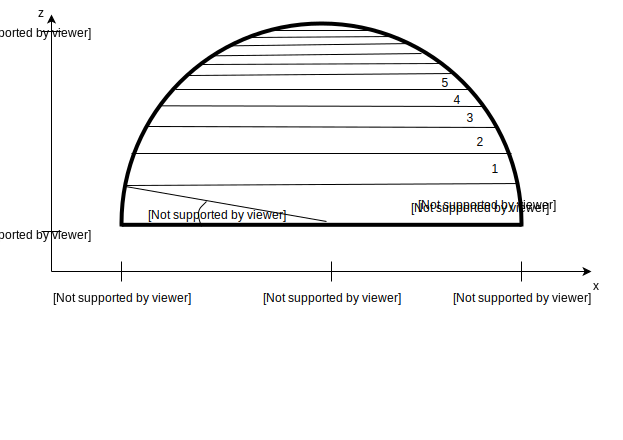
\includegraphics[width=0.7\columnwidth]{Images/PrismCl-Rings.png}
    \caption{rings_FromSide}
    \label{fig:rings_FromSide}
\end{figure}

\begin{figure}
    \includegraphics[width=0.7\columnwidth]{Images/PrismCl-RingsFromTop.png}
    \caption{rings_FromTop}
    \label{fig:rings_FromTop}
\end{figure}

\begin{figure}
    \includegraphics[width=0.4\columnwidth]{Images/PrismCl-RingAngle.png}
    \caption{ringAngle}
    \label{fig:ringAngle}
\end{figure}


This hemisphere is separated into rings. Each ring covers the threshold angle $\phi$ in $z$-direction and is visualized in Figure \ref{fig:rings_FromSide} and Figure \ref{fig:rings_FromTop}. Each normal is sorted into a ring by its correlating angle $\alpha$ which is used to determine the ring index. It is proporional to its coordinates as demonstraded in Figure \ref{fig:ringAngle}: the angle between $\vec{n}$ and $(x,y,0)$:

\begin{equation*}
\begin{split}
    \sin{\alpha} & = \frac{z}{ \sqrt{x^{2} + y^{2}} } \\
    => \alpha  & = \arcsin{ \frac{z}{ \sqrt{x^{2} + y^{2}} } }
\end{split}
\end{equation*}


The angle $\alpha$ is represented as a multiple of the threshold angle $\phi$ to get the actual ring index $I_{Ring}$:

\begin{equation*}
    I_{Ring} = \floor*{
                    \arcsin{
                        \frac{z}{ \sqrt{ x^{2} + y^{2} } }
                    }
                    / \phi
                }
\end{equation*}

The maximum angle is 90° (normal $ = (0,0,1)$). Consequently the maximum ring index $I_{MaxRing}$ is calculated as follows:

\begin{equation*}
    I_{MaxRing} = \floor*{
                    \frac{\pi}{2}
                    / \phi
                  }
\end{equation*}



The angle in the middle of each ring ${\alpha}_{I_{Ring}}$ consequently depends on index and threshold:

\begin{equation}
\label{equ:AlphaIRing}
    {\alpha}_{I_{Ring}} = (I_{Ring} + 0.5) * \phi \qquad \forall{ I_{Ring} \in [0, I_{MaxRing}] }
\end{equation}



Figure \ref{fig:middleZ} implies the calculation of the corresponding middle $z$ value $z_{I_{Ring}}$: We create a normal $\vec{a}_{I_{Ring}}$ with a fixed $y$ value of 0 that forms the angle ${\alpha}_{I_{Ring}}$ with the unit vector in x direction $\vec{v}_{x}$. Consequently all normals that lie in the middle of a ring ($\alpha = {\alpha}_{I_{Ring}}$) have the $z$ value $z_{I_{Ring}}$.

\begin{figure}
    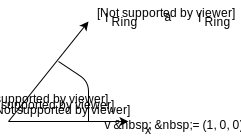
\includegraphics[width=0.5\columnwidth]{Images/PrismCl-MiddleZ.png}
    \caption{middleZ}
    \label{fig:middleZ}
\end{figure}

\begin{equation}
\label{equ:VecX}
    \vec{v}_{x} = (1, 0, 0)
\end{equation}

\begin{equation}
\begin{split}
    \label{equ:VecA}
    \vec{a}_{I_{Ring}} = (x_{a}, 0, z_{I_{Ring}}) \qquad  & \forall{ I_{Ring} \in [0, I_{MaxRing}] } \\
    & with \vert \vec{a}_{I_{Ring}} \vert = 1
\end{split}
\end{equation}

\begin{equation}
    \label{equ:XA}
    \cos{{\alpha}_{I_{Ring}}} = \frac{ \vec{v}_{x} * \vec{a}_{I_{Ring}} }{ \vert \vec{v}_{x} \vert * \vert \vec{a}_{I_{Ring}} \vert }
    \stackrel{(\ref{equ:VecX}) + (\ref{equ:VecA})}{=} \vec{v}_{x} * \vec{a}_{I_{Ring}}
    \stackrel{(\ref{equ:VecX}) + (\ref{equ:VecA})}{=} x_{a}
\end{equation}

\begin{equation}
\label{equ:ZIRing}
\begin{split}
    1 & = \vert \vec{a}_{I_{Ring}} \vert \stackrel{(\ref{equ:VecA})}{=} \sqrt{ x_{a}^{2} + z_{I_{Ring}}^{2} } \\
    => z_{I_{Ring}} & = \sqrt{1 - x_{a}^{2}}
    \stackrel{(\ref{equ:XA})}{=} \sqrt{1 - cos^{2}{{\alpha}_{I_{Ring}}}}
\end{split}
\end{equation}


Each ring is seperated into buckets which cover the threshold angle $\phi$ as shown in Figure \ref{fig:PrismCl-buckets}. Therefore the onto the xy-plane projected angle $\gamma$ needs to be calculated which differs from ring to ring. This is shown in Figure \ref{fig:projection} and leads to this calculation:

\begin{figure}
    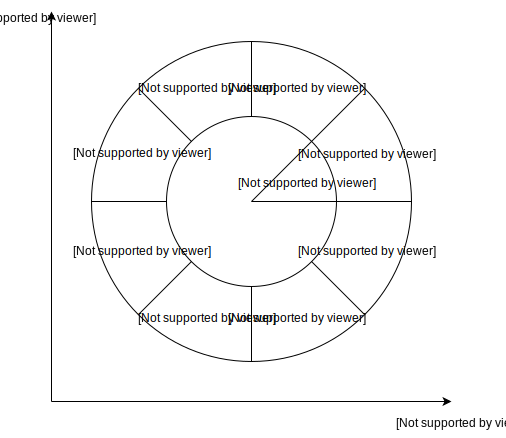
\includegraphics[width=0.7\columnwidth]{Images/PrismCl-buckets.png}
    \caption{buckets}
    \label{fig:PrismCl-buckets}
\end{figure}


\begin{figure}
    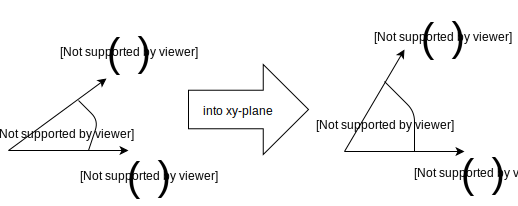
\includegraphics[width=1.0\columnwidth]{Images/PrismCl-Projection.png}
    \caption{projection}
    \label{fig:projection}
\end{figure}


$ \vec{a}_{I_{Ring}}' $ is the projection of $\vec{a}_{I_{Ring}} $:


\begin{equation}
    \label{equ:VecAStrich}
    \vec{a}_{I_{Ring}}' = (x_{a}, 0)
\end{equation}

$ \vec{b}_{I_{Ring}} $ spans the threshold angle $\phi$ with $ \vec{a}_{I_{Ring}} $ and has the same $z$ value $z_{I_{Ring}}$:

\begin{equation}
    \vec{b}_{I_{Ring}} = (x_{b}, y_{b}, z_{I_{Ring}}) \qquad with | \vec{b}_{I_{Ring}}| = 1
    \label{equ:VecB}
\end{equation}

The corresponding projected vector $ \vec{b}_{I_{Ring}}' $:

\begin{equation}
    \vec{b}_{I_{Ring}}' = (x_{b}, y_{b})
    \label{equ:VecBStrich}
\end{equation}

Due to the mentioned conditions the coordinates of $ \vec{b}_{I_{Ring}} $ are calculated as follows:


\begin{equation}
    \label{equ:Projection1}
    \cos{\phi} = \frac{\vec{a}_{I_{Ring}} * \vec{b}_{I_{Ring}}}{|\vec{a}| * |\vec{b}|} = \vec{a}_{I_{Ring}} * \vec{b}_{I_{Ring}} \stackrel{(\ref{equ:VecA}) + (\ref{equ:VecB})}{=} x_{a}_{I_{Ring}} * x_{b}_{I_{Ring}} + z_{I_{Ring}}^{2}
\end{equation}

\begin{equation}
    \label{equ:XB}
   (\ref{equ:Projection1}) => x_{b} = \frac{ \cos{\phi} - z_{I_{Ring}}^{2} }{ x_{a} }
\end{equation}

\begin{equation}
\begin{split}
    \label{equ:YpsilonB}
    & 1 = |\vec{a}_{I_{Ring}}| = |\vec{b}_{I_{Ring}}| \\
    & => \sqrt{ x_{a}^{2} + z_{I_{Ring}}^{2} } = \sqrt{ x_{b}^{2} + y_{b}^{2} + z_{I_{Ring}}^{2} } \\
    & => y_{b} = \sqrt{ x_{a}^{2} - x_{b}^{2} }
\end{split}
\end{equation}


The angle ${\gamma}_{I_{Ring}}$ which is used to separate a ring into buckets is calculated with the projected vectors $ \vec{a}_{I_{Ring}}' $ and $ \vec{b}_{I_{Ring}}' $ :

\begin{equation}
\begin{split}
    \cos{{\gamma}_{I_{Ring}}}& = \frac{\vec{a}_{I_{Ring}}' * \vec{b}_{I_{Ring}}'}{|\vec{a}_{I_{Ring}}'| * |\vec{b}_{I_{Ring}}'|}
    = \frac{ x_{a} * x_{b} }{ x_{a} * \sqrt{  x_{b}^{2} +  y_{b}^{2} } } \\
    & \stackrel{(\ref{equ:YpsilonB})}{=} \frac{ x_{a} * x_{b} }{ x_{a} * \sqrt{  x_{b}^{2} - x_{b}^{2} +  x_{a}^{2} } }
    = \frac{ x_{a} * x_{b} }{ x_{a} * x_{a} }
    = \frac{ x_{b} }{ x_{a} } \\
    & \stackrel{(\ref{equ:XB})}{=} \frac{ \cos{\phi} - z_{I_{Ring}}^{2} }{ x_{a}^{2} }
    \stackrel{(\ref{equ:XA})}{=} \frac{ \cos{\phi} - z_{I_{Ring}}^{2} }{ \cos^{2}{{\alpha}_{I_{Ring}}} } \\
    & \stackrel{(\ref{equ:ZIRing})}{=} \frac{ \cos{\phi} - ( 1 - cos^{2}{{\alpha}_{I_{Ring}}} ) }{ \cos^{2}{{\alpha}_{I_{Ring}}} }
    = \frac{ \cos^{2}{{\alpha}_{I_{Ring}}} }{ \cos^{2}{{\alpha}_{I_{Ring}}} } + \frac{ \cos{\phi} - 1 }{ \cos^{2}{{\alpha}_{I_{Ring}}} } \\
    & \stackrel{(\ref{equ:AlphaIRing})}{=} 1 + \frac{ \cos{\phi} - 1 }{ \cos^{2}{( (I_{Ring} + 0.5) * \phi )} } \\
    => {\gamma}_{I_{Ring}} & = \arccos{( 1 + \frac{ \cos{\phi} - 1 }{ \cos^{2}{( (I_{Ring} + 0.5) * \phi )} } )}
\end{split}
\end{equation}


The corresponding angle $ \beta $ of a normal $ \vec{n} $ is calculated with use of the unit vector in x direction $ \vec{v_{x}'} $. This angle needs to be adapted in case $ y < 0 $ since the maximum angle between two vectors is 180° and we want to cover a complete circle:

\begin{equation}
\begin{split}
    \cos{\beta} & = \frac{\vec{n}' * \vec{v_{x}'}}{|\vec{n}'| * |\vec{v_{x}'}|} = \frac{x}{\sqrt{x^{2} + y^{2}}} \\
    => \beta & = \begin{cases}
        \arccos{ \frac{x}{\sqrt{x^{2} + y^{2}}} }, & y \geq 0 \\
        2 \pi - \arccos{ \frac{x}{\sqrt{x^{2} + y^{2}}} }, & y < 0
    \end{cases}
\end{split}
\end{equation}

The angle $ \beta $ is represented as a multiple of the $ \gamma $ angle to get the bucket index $ I_{Bucket} $:

\begin{equation}
    I_{Bucket} = \floor{\frac{\beta}{ {\gamma}_{I_{Ring}} }}
\end{equation}

Consequently the maximum bucket index is calculated with the maximum angle of 360°:

\begin{equation}
    I_{MaxBucket} = \floor{\frac{2 \pi}{ {\gamma}_{I_{Ring}} }}
\end{equation}



\subsubsection{Implementation}

\myNotes{TODO: Klassendiagramm}

The \emph{PrismClassifier} works on \emph{shapes} from the \emph{ClassifierGraph} and should also take account of \emph{planes} in future development. Therefore it depends on the \emph{PlaneClassifier}. It returns a set of \emph{prisms} and uses \emph{PrismShapeNormalsBuckets} to check shapes for parallelism.

\paragraph{PrismClassifier}

\begin{listing}[!h]
\centering
\begin{minted}[
linenos, breaklines
]{coffeescript}
run: ->
    return new Promise( (resolve) =>
        buckets = new PrismShapeNormalsBuckets(_angleThreshold)

        @_putIntoBuckets @shapes, buckets

        prisms = @_detectPrisms @shapes, buckets

        log.debug("PrismClassifier found " + prisms.length + " prisms")

        resolve(prisms)
    )
\end{minted}
\caption{run method of the PrismClassifier}
\label{lst:PrismClassifierRun}
\end{listing}

Listing \ref{lst:PrismClassifierRun} shows the implementation of the \emph{PrismClassifier} run method:

At first the normal buckets are initialised with an angle threshold as described in section \emph{Bucket System}. These values are stored in the global config with \emph{\_angleThreshold} $ = 0.15 $  ( = 8.6\textdegree, previously labeled $\phi$) so shapes with an angle  of 8.6\textdegree \hspace{1pt} will be considered parallel.

Then all shapes are put into the corresponding buckets. This is done by iterating over all shapes and passing them to the bucket system which handles the classification on its own.

Next we iterate over all shapes again while requesting the potential parallel shapes from the bucket system. The shapes are checked with the given threshold and a \emph{prism} is created in case of parallelism.

At the end a set of all prisms is returned which can be used for further primitive classification.


\paragraph{PrismShapeNormalsBuckets}

\emph{PrismShapeNormalsBuckets} is based on the specification in section \ref{sec:PrismBucketSystem} Bucket System: It divides a hemisphere into rings with buckets and is initialised with the angle threshold.

The constructor saves the angle threshold, instantiates the rings as a \emph{javascript map} and calculates the maximum ring index $I_{MaxRing}$.

It provides two functions used by the classifier: \\
\emph{push} and \emph{getShapesToCheckAndDeleteThisOne}.

\emph{push} takes a \emph{shape} and puts it in the corresponding ring. At first it transforms its normal into the hemisphere. Then the ring index $ I_{Ring} $ is calculated. If the ring is not initialised yet it gets created and \emph{ring.push(shape)} is called to sort the \emph{shape} into the corresponding bucket.

\emph{getShapesToCheckAndDeleteThisOne} takes a shape and removes it from the bucket system because it will be checked for all possible prisms by the classifier and should not be returned as a potential parallel shape in another pass. Then it returns an array of all shapes lying in the same and the surrounding buckets: It requests the corresponding buckets from the ring with the shape's ring index $ I_{Ring} $ and the ring above and beneath.

While determining the surrounding rings following special cases need to be considered:

First: The ring with the maximum index $I_{MaxRing}$ is only adjacent to the ring underneath, because it is the highest ring on top of the hemisphere. It is not separated into different buckets and serves as a single bucket which is adjacent to all buckets in the ring underneath.

Second: The ring with index 0 "is adjacent to itself" because the unit sphere got transformed into a hemisphere. Therefore the buckets 180° around have to be taken into account for parallelism checks. Let's take two normals with the same x, y coordinates and a negated z value that span an angle smaller $ \phi $: $\vec{n_{1}} = (x, y, z)$ and $\vec{n_{2}} = (x, y, -z)$ with $z > 0$. Consequently $\vec{n_{1}}$ naturally lies in ring 0 and $\vec{n_{2}}$ gets negated to fit into the hemisphere. The negated normal is $\vec{n_{2}}' = (-x, -y, z) $ and lies also in ring 0 but in the opposite bucket (180° away).


\paragraph{Ring}

A \emph{Ring} contains buckets as a javascript map and is initialized with an index $ I_{Ring} $ and the angle threshold $ \phi$. With these the angle $ \gamma $ and the maximum bucket index $ I_{MaxBucket} $ are calculated as described in section \ref{sec:PrismBucketSystem} Bucket System. It provides the methods \emph{push}, \emph{get}, \emph{getAndSurrounding}, \emph{getAll}, \emph{delete} and \emph{getSize}

The method \emph{push} sorts a given shape into the corresponding bucket. \emph{get} returns all shapes of a bucket with a given index, \emph{getAndSurrounding} returns the same and additionaly the two neighboring buckets while \emph{getAll} returns all shapes that lie in that ring. With \emph{delete} a given shape is removed from the ring and \emph{getSize} returns the amount of shapes that lie in that ring.


\paragraph{MaxRing} The \emph{MaxRing} is only instanced once and is the ring with index $ I_{RingMax} $. It provides the same methods as a \emph{Ring} but with adapted behaviour.

\paragraph{Prism}

A \emph{Prism} contains two parallel shapes that span a prism. In future work this should be extended by the lateral surface which is not handlet yet.

\subsubsection{Future Work}
\label{sec:PrismFutureWork}

\paragraph{Planes} \emph{Planes} from the \emph{PlaneClassifier} should be taken into account in addition to the shapes. Ideally the \emph{PlaneClassifier} detects noisy planes that are not represented as shapes. Therefore a better approximation of the original model could be achieved.

\paragraph{Lateral Surface} The lateral surface of the prism has yet to be identified and added to the prism structure. This is needed for further operations and more specific classifications of the prism. For example for classifying a cube the surrounding sides have to be known.

\paragraph{Scoring} Prism scoring is not implemented yet. To rate a prism the actual angle between the two nearly parallel shapes have to be considered. If scoring is implemented the angle threshold for parallelism can be adjusted to a much higher value while big variations to 0° will be reflected in the score.


\end{document}

\cleardoublepage

%\part{Plates}
\subfile{Chapters/05-Plates}
%\documentclass[../ClassicThesis.tex]{subfiles}
\begin{document}

%************************************************
\chapter{Plates}\label{ch:plates}
%************************************************

\section{Overview of approaches for finding plates}

There are multiple approaches for finding plates contained in a 3D-mesh. The first, called inherent plates, requires the plates to be actually modeled in the mesh with both a top and a bottom side. The second approach, extruded plates, uses the mesh surface to extrude plates into the object. While this method works on more meshes then the inherent approach, it can produce doubled plates if they are modeled in the mesh. The third approach is to stack plates, creating a filled approximation of the mesh.

\section{Prerequisites for finding plates}

coplanar / shapesfinder / holedetection

\subsection{Coplanar Faces}

The algorithm for finding coplanar faces requires the models to be stored as a face-vertex mesh. This is calculated by Meshlib, the library used for importing models. In a face-vertex mesh, faces only store their vertices' indices, with the vertices being stored in a different lookup table. This allows for easier adjacency checks - only the vertex indices have to be compared. Additionally, the face normals are stored in an array, in the same order as in the face list.

Now, two more lookup tables are added: One contains all edges (stored as a sorted pair of vertex indices) belonging to each face, while the second one allows looking up the faces adjacent to an edge. Both lists can be created in one single pass. 

\begin{listing}[ht]
\begin{minted}[
linenos
]{coffeescript}
setupFaceEdgeEdgeFaceLookup: ->
  for faceIndex in [0...faceCount]
    # Determine the ordering of vertices (this avoids double edges)
    { min_vertex
      mid_vertex
      max_vertex } = @findMinMidMaxVertex()
    # Register which edges this triangle uses.
    @addEntryToEdgeFaceMap(min_vertex, mid_vertex, faceIndex)
    @addEntryToEdgeFaceMap(mid_vertex, max_vertex, faceIndex)
    @addEntryToEdgeFaceMap(min_vertex, max_vertex, faceIndex)
    # Set the edges that make up this triangle.
    @faceVertexMesh.faceToEdges[faceIndex] = [
      [min_vertex, mid_vertex]
      [mid_vertex, max_vertex]
      [min_vertex, max_vertex]
    ]
\end{minted}
\caption{Simplified lookup table generation.}
\label{lst:coffeescript}
\end{listing}

Afterward, the faces are grouped. This in done by iterating over all faces. When a face is found which hasn't been visited yet, a new face group is started. Now all of the face's edges are pushed to a queue, along with the current face index.

\begin{listing}[ht]
\begin{minted}[
linenos
]{coffeescript}
for faceIndex in [0...faceCount] when not faceVisited[faceIndex]
  faceGroup = [faceIndex]
  faceGroupIndex = faceGroups.length
  outerEdgeGroup = []
  groupNormal = @faceVertexMesh.getFaceNormal(faceIndex)
  faceVisited[faceIndex] = true
  # connect the adjacent faces
  edgeQueue = []
  adjacentEdges = @faceVertexMesh.getEdgesFromFace(faceIndex)
  for edge in adjacentEdges
    edgeQueue.push({ edge, faceIndex })
  @traverseAdjacentFaces(...)
\end{minted}
\caption{Iteration over faces with creation of new face groups.}
\label{lst:coffeescript}
\end{listing}

There are multiple important variables being set here: First, we have the new face group, containing only the current face. Next, we have the index of the face group, used for creating a face to face group lookup table. The outerEdgeGroup contains all edges surrounding the group, wich allows the creation of a shape containing the face group. The group's normal vector is initialized with the current face's normal vector. Lastly, the current face is marked as visited in order to avoid checking it multiple times.

After the edges have been pushed in the queue, we start working on the it:

\begin{listing}[ht]
\begin{minted}[
linenos
]{coffeescript}
traverseAdjacentFaces: tco (
    edgeQueue,
    faceVisited,
    faceGroup,
    faceGroupIndex,
    outerEdgeGroup,
    groupNormal
  ) ->
    if edgeQueue.length is 0
      return

    { edge, faceIndex } = edgeQueue.shift()
    faceNormal = @faceVertexMesh.getFaceNormal(faceIndex)

    # get the faces from the edge and choose the one thats not the current one
    adjacentFaces = @faceVertexMesh.getFacesFromEdge(
      edge[0]
      edge[1]
    )

    nextFaceIndex =
      if adjacentFaces[0] is faceIndex
      then adjacentFaces[1]
      else adjacentFaces[0]
    nextFaceNormal = @faceVertexMesh.getFaceNormal(nextFaceIndex)

    if @isAngleZero(faceNormal, nextFaceNormal)
      if not faceVisited[nextFaceIndex]
      # if the adjacent face is coplanar and wasn't visited yet
      # add to group, mark as visited, check adjacent faces
        faceGroup.push(nextFaceIndex)
        groupNormal.add(nextFaceNormal)
        @faceToFaceGroup[nextFaceIndex] = faceGroupIndex
        faceVisited[nextFaceIndex] = true

        adjacentEdges = @faceVertexMesh.getEdgesFromFace(nextFaceIndex)
        for edge in adjacentEdges
          edgeQueue.push({ edge, faceIndex: nextFaceIndex })
    else
      # the edge is an outer edge for this coplanar group
      # in that case, don't check if the face was already visited
      outerEdgeGroup.push(edge)

    @recur(
      edgeQueue
      faceVisited
      faceGroup
      faceGroupIndex
      outerEdgeGroup
      groupNormal
    )
\end{minted}
\caption{Iteration over faces with creation of new face groups.}
\label{lst:coffeescript}
\end{listing}

\subsection{Shape Finder / Deus}



\subsection{Hole Detection / Dimitri}

sdfjkljklsdfsdfjkl

\section{Finding inherent plates}

In order to find inherent plates in a mesh, the first step is to find all shapes which are parallel and check if the distance between them fits one of the given plate thicknesses.

\begin{listing}[ht]
\begin{minted}[
linenos
]{coffeescript}
candidates = []
for shape1, index1 in shapes
    for shape2, index2 in shapes when index1 < index2
        if normals parallel and surfaces facing apart
            if distance between shape1, shape2 in plate thicknesses
                candidates.push { shape1, shape2 }
return candidates
\end{minted}
\caption{Plate candidate pseudo code.}
\label{lst:coffeescript}
\end{listing}

While the testing for normal parallelism is done with built-in vector functions, the check if the surfaces are facing apart uses a vertex of each of the surfaces and calculates the angle of the resulting vector to one of the normals. If this angle is smaller than 90\textdegree, the surfaces are indeed facing apart. The distance between the surfaces is calculated by creating a three.js plane from one of the shapes and computing the plane-to-point distance towards one of the other shape's points.

After finding these plate candidates, the shapes which plane's distance to the origin (the z-value of all vertices when laid into the x-y-plane) is smaller is selected as the base shape of the plate. Now, the intersection of both shapes is calculated. This is done by using the already calculated mapping of vertices into the x-y-plane. The resulting intersection is transformed back into 3D-space using the rotation matrix of the base shape. With the resulting shapes, plates are created.

% \begin{center}Listing XYZ: Plate creation
% \begin{lstlisting}
% shape2CloserToOrigin = abs(shape2.zValue) < abs(shape1.zValue)
% polygon1 = create2DPolygon(shape1)
% polygon2 = create2DPolygon(shape2)
% intersection = polygon1.intersect polygon2
% shapes = parseToShapes(intersection)
% plates = parseToPlates(shapes)
% return plates
% \end{lstlisting}
% \end{center}

This step uses the jsclipper library for intersecting the shapes. After parsing them into the library's polygon class, they can be easily clipped, resulting in a list of intersections which can be parsed back into shapes. The plate creation is based on the previously selected base shape. While the calculated intersection is used as the shape of the plate, the thickness is computed by subtracting the base shape's z-value from the other shape's z-value. Additionally, the base shape's z-value is used as plane constant.

\section{Extruding plates}

blabla

\section{Removing contained plates / Dimitri}

dfgdfgdfgdfgdfg

\section{Stacking plates}

blablabla

% Hey Lukas hier ist Klara, habe eine alternative methode für algorithms darstellen, die finde ich persönlich übersichtlicher.
% HIer ein Beispiel:
% \begin{algorithm}[H]
% \DontPrintSemicolon
% 	\KwData{this text}
% 	\KwResult{how to write algorithm with \LaTeX2e }
% 	initialization\;
% 	\While{not at end of this document}{
% 	read current\;
% 	\eIf{understand}{
% 	go to next section\;
% 	current section becomes this one\;
% 	}{
% 	go back to the beginning of current section\;
% 	}
%      \For{all I know}{
%      look at this link to learn more about \LaTeX2e:\;
%      http://ctan.space-pro.be/tex-archive/macros/latex/contrib/algorithm2e/doc/algorithm2e.pdf\;
%      }
% 	}
%    \caption{How to write algorithms}
% Kannst ja mal überlegen, wir sollten uns aber auf eins von beiden einigen

% \end{algorithm}

\end{document}
\cleardoublepage

%\part{Graph}
\subfile{Chapters/06.1-Graph}
%\documentclass[../ClassicThesis.tex]{subfiles}
\begin{document}
%************************************************
\chapter{Adjacency Plategraph / Klara}\label{ch:graph}
%************************************************

% Use active Voice (we do….)
% Ein Gedanke pro Paragraph
% Terminologie anpassen über alle Arbeiten hinweg (was ist eine Plate für alle…)
% Jeder sollte eine kleine Related Work section haben
% Erklärungen zu warum dieser Algorithmus genutzt wurde und nicht ein anderer + limitations des gewählten Algorithmus
% Hübsche Bildchen zum anschaulichen Erklären!! (ebenfalls konsistent halten: gleich geformte labels etc.)
% FROM SOLUTION TO PROBLEM /DISCUSSION
% EXPLAIN ALL VARIABLES ETC.!!!

% 1. Was macht es inhaltlich
% 2. Was kann/tut der Graph überhaupt?


% \paragraph{Why is this part necessary?}
On the basis of the graph we can create connectors for plates in a later step ( \ref{ch:joints}). Depending on angles and neighborhood relationships an adequate connector type can be chosen.
% for what? to figure out joint connections?

% \paragraph{What is being achieved in this Chapter?}
In this step we analyse the spatial arrangement of plate objects in 3D-space to create a graph structure which tracks the adjacency. The plates to be analysed are found in the previous step \ref{ch:plates}. Two or more plates are adjacent to another when at least one side touches or overlaps with another plate. In addition, the angles in between the plates are measured. 


% WHAT IS WITH THE 3D SNIPPETS??? DO THEY STILL EXIST?

% \paragraph{Chosen Graph Class Structure}
The graph always holds a list of all found plates and their neighbors. A plate is just one possible object to be listed. Other graph nodes can be left over 3D snippets which will have to be handled when all plates have been correctly connected.\\
For iterating over the graph we traverse all edges of the graph which also hold the important neighborhood parameters such as angle and the line at which nodes intersect.\\\* \\
\hspace*{-1.8cm}
\includegraphics[width=1.3\columnwidth]{Images/GraphStructure.png}


\section{Analysing spatial arrangement}
% \subparagraph{requirements for running the algorithm}
% unnecessary??
As a prerequisite the step \ref{ch:plates} needs to find inherent or create extruded plates first. Afterwards the plane-plane intersections of all combinations of both sides of the plates are computed which results in up to four intersection lines. In preparation for the joint generation step \ref{ch:joints} we truncate the inner intersection lines which would otherwise overlap with adjacent plate intersections.

\subsection{Finding intersections}
% \subparagraph{concrete explanation, functions used/example code etc.}
When two planes intersect there is an intersection line. Since we work with plates which equal 2 parallel planes we expect to find up to 4 intersection lines.\\
Firstly, we retrieve the direction vector(\emph{dir}) of any intersection line between two plates by calculating the cross vector of both normals.\\
% TODO: include citation
In order to retrieve all possible intersection lines of two plates we calculate four possible plane-plane intersections \cite{planePlaneIntersection} of 
\begin{itemize}
\item the two main sides of the plates
\item the two parallel sides of the plates
\item one main and one parallel side 
\item and the other way around
\end{itemize}
\*\\
First, a possible position vector has to be found which lies on both planes.
\\\*\\
\emph{Plane constants:} $d_1, d_2$\\
\emph{Normals:} $n_1, n_2$
$$ p = \frac{d_1 * n_{2}^{2} - d_2 * (n_1 * n_2)}{n_{1}^{2} * n_{2}^{2} - (n_1 * n_2)^{2}} * n_1 + \frac{d_2*n_1^2 - d_1*(n_1 * n_2)}{n_1^2 * n_2^2 - (n_1 * n_2)^2} * n_2 $$

On the basis of a position vector an intersection line can be computed.
% TODO: make this nicer
$$ line = p*x + dir$$

Now that all lines are found we have to test if the lines actually go through both plates. In addition, this step retrieves the exact start and end points of the line segment that defines the intersection of both plates.\\
In order to find the boundaries of the lines we calculate the intersections of the lines with all boundary edges of the plates.\\
\includegraphics[width=.5\columnwidth]{Images/HeadAllBoundaries.png}

\subsection{Determine angles between plates}
In order to generate nicely fitting joints in the following step and for grouping plates the angles are necessary.\\
Firstly, we determine the angle between the according planes.\\
plane normals: u, v\\
angle between planes: $\theta$
$$ cos(\theta) = \frac{u \cdot v}{|u| * |v|}$$
But we are not talking about infinitely large planes instead we want the angle which is enclosed by the finitely large plates. Therefore we need to adjust the angle in some cases dependent on the direction in which the normals are pointing.
% figure which shows when angle is right, but also one case when it is not right
\begin{figure}[h]

\includegraphics[width= 1\columnwidth]{Images/anglesExamplesSmall.png}
\caption{(a) The angle between the plates' normals correspond with the angle $\gamma$ between the plates. (b) The angle between the plates' normals is in this case an adjacent angle to the requested angle $\gamma$.}
\end{figure}

In order to find out in which cases the angle has to be adjusted we check for two properties.\\
Firstly, there is the question which of the sides of the plates intersect. A plate is defined by a 2D-shape which is called main side. The other side which exists due to a specified thickness of the plate is called parallel side.\\
Additionally, we look at the direction of the normals. The direction is positive when it is directed from the main to the parallel side and negative otherwise.\\
For an angle to be in need to be adjusted the following conditions need to be satisfied.
\begin{itemize}
    \item The two plates touch with the same type of side 
    \item[] AND
    \item Their directions are both positive OR both negative
\end{itemize}



\subsection{Truncating intersection lines}
Now that all lines are known we need to shorten the lines so that no other lines overlap with it. If this step is missing then the following step for creating joints will run in to problems that the joints overlap each other.\\
If we now have a look at only the inner intersections of plates in a model we can identify the overlaps.
\begin{figure}[t]
\includegraphics[width=.5\columnwidth]{Images/HeadInnerBoundaries.png}
\caption{The inner boundaries of the plates overlap. In the next step when joints will be created they are only supposed to be on the inner part of the line. Therefore the lines have to be truncated.}
\end{figure}
\*\\
\begin{algorithm}[H]
	\DontPrintSemicolon
	\KwData{lines}
	\KwResult{truncated lines}
	initialize variables here\;
    \For{line$\_$pair in lines}{
    	line1 = line$\_$pair[0]\;
        line2 = line$\_$pair[1]\;
        point = lineLineIntersection(line1, line2)\;
        \If{isPointOnLine(point, line1) and isPointOnLine(point, line2)}
        {
       		\tcp{linesegments actually cross}
       		startSegmentLine1 = new Line(point, line1.start)\;
            endSegmentLine1 = new Line(point, line1.end)\;
            startSegmentLine2 = new Line(point, line2.start)\;
            endSegmentLine2 = new Line(point, line2.end)\;
            \tcp{the shorter part of each line is discarded}
			\eIf{startSegmentLine1.distance() $>$ endSegmentLine1.distance()}{
				\eIf{startSegmentLine2.distance() $>$ endSegmentLine2.distance()}{
				return \{
                    	endSegmentLine1\;
                        endSegmentLine2
                    \}
				}{
                    return \{
                    	endSegmentLine1\;
                        startSegmentLine2
                    \}
				}
			}{
			return \{
                	startSegmentLine1\;
                    startSegmentLine2
                \}
			}	      
        }
    }
   	\caption{Truncate lines}
\end{algorithm}



\section{Alternative Solutions}
\subsection{Dustin: how he did it}
\subsection{Dustins wrong angles}
he didnt actually specify how he calculated the angles...
\subsection{Down sides}
\subsection{Whats better now?}

\section{How we got there}
\subsection{Floating Point inaccuracy}
\subsection{Bruteforce finding lines}
\subsection{different line intersection algorithms}

\section{Future work}
- find out if model is assemblable in the end



% Dummy algorithm:\\
% \begin{algorithm}[H]
% 	\DontPrintSemicolon
% 	\KwData{input Data}
% 	\KwResult{result Data}
% 	initialize variables here\;
%    \caption{Name of Algorithm}

% \end{algorithm}



% \begin{algorithm}[H]
% \DontPrintSemicolon
% 	\KwData{this text}
% 	\KwResult{how to write algorithm with \LaTeX2e }
% 	initialization\;
% 	\While{not at end of this document}{
% 	read current\;
% 	\eIf{understand}{
% 	go to next section\;
% 	current section becomes this one\;
% 	}{
% 	go back to the beginning of current section\;
% 	}
%      \For{all I know}{
%      look at this link to learn more about \LaTeX2e:\;
%      http://ctan.space-pro.be/tex-archive/macros/latex/contrib/algorithm2e/doc/algorithm2e.pdf\;
%      }
% 	}
%    \caption{How to write algorithms}

% \end{algorithm}






\end{document}
\cleardoublepage

%\part{Joints}
\subfile{Chapters/06.2-Joints}
%\documentclass[../ClassicThesis.tex]{subfiles}
\begin{document}

%************************************************
\chapter{Joint Computation}\label{ch:joints}
\newcommand{\TODO}[1]{\textcolor{red}{\\ \textbf{TODO:} #1 \\}}
%************************************************

% Use active Voice (we do….)
% Ein Gedanke pro Paragraph
% Terminologie anpassen über alle Arbeiten hinweg (was ist eine Plate für alle…)
% Jeder sollte eine kleine Related Work section haben
% Erklärungen zu warum dieser Algorithmus genutzt wurde und nicht ein anderer + limitations des gewählten Algorithmus
% Hübsche Bildchen zum anschaulichen Erklären!! (ebenfalls konsistent halten: gleich geformte labels etc.)

\section{Joint computation}
\TODO{buy green and orange (or at least two different colors) of acrylic for demo objects and pictures in the paper}
\paragraph{Overview Paragraph: what will be achieved, why is it necessary}
When an object consisting of multiple parts is lasercutted it needs to have connectors. Those can be elements like screws, nails and glue. Or the plates already come along with connectors. Those can be for example fingerjoints which, when well calibrated, do not need any external material to hold together. \\
Whenever possible we want to provide connections like that because a user needs less effort, when components work directly out of the lasercutter. This is why we provide three types of joints which are added to the determined plates.

\subsection{Volume based clipping}
Before joints can be added to the plates we have to prepare them. We cut the shapes back so that the joints do not overlap with the other plate.
\paragraph{prerequisite: plategraph intersection lines}
As seen before in the step [plateGraph] up to four intersectionlines will have been calculated.\\
Two of them lie both on one side of the plate and the other two belong to the second side. The two lines on one side build a rectangle when their ends are connected. We use those two rectangles to cut out of the plate what will get fingerjoints.\\
%\textbf{TODO: Insert image of the four lines, with the two rectangles marked.}\\
\includegraphics[width=\columnwidth]{Images/10-joints-clippingPlate.jpg}\\
There are cases when not all four lines are actually a plate intersection but only a plane intersection. \\
%\textbf{TODO: Image of plates which result in not 4 intersections.}\\
\includegraphics[width=\columnwidth]{Images/10-joints-casesOfLines.jpg}\\
In this case the infinitifly long plane intersection line will be clipped to match the length of the existing plate intersections. This yields two rectangles as well, which can then be used for clipping the shapes of the plates.



\section{building joints}
The general procedure of creating joints is achieved in three steps: First we calculate how many female and male joints fit onto the intersection. Then the retrieved joints are placed at the intersectionline and finally the shapes are merged to result in the original plate with joints.
\begin{enumerate}
    \item buildAlignedJointTemplates\\
        \paragraph{jointCount}
        We need to know how many joints we have to place onto the intersection. We call this 'jointCount' which describes the number of all joints to fit on the line including the male and female joints. Since all joint types have equal widths for female and male joints we divide the length of the line by the width of a joint.
        \paragraph{adjustJointWidth}
        But this calculation has to be rounded which means the number of joints just found might not fill the complete length of the line after all. Therefore we adjust the width so that the joints will be evenly spread without leaving space on either end of the line.
        Now that we know how the joints will look like and how many we need it is time to find out how to distribute them.\\
        We defined that when there is an even number of joints, the middle joint will be male and twice as thick as normally.\\
        %\textbf{TODO: provide image of the two cases: even and odd number}
        \includegraphics[width=\columnwidth]{Images/10-joints-evenOddJointCount.jpg}
        \paragraph{computeMaleJointsPerSide} %number only
        On both sides of the middle joint will be an equal number of male joints. How many depends on the jointCount. An even jointCount means 2 joints less and odd means one joint less on the sides because the middle joint will be created seperately. Since the jointCount specifies the number of all joints, male and female we have to divide by two to get the number of male joints only and then divide by two once more to achieve the seperation into the two sides.\\
        maleJointsPerSide = 
        \begin{cases} 
        (jointCount - 2) / 4, & jointCount $ \% 2 == 0 $ \\ 
        (jointCount - 1) / 4, & jointCount $ \% 2 == 1 $
        \end{cases}
            \paragraph{buildJointsForEven / Odd count}
            Finally, we can start placing the middle joint and distributing as many joints as just calculated on either side of it evenly with leaving enough space inbetween the joints for a female one to fit in.\\
            % \textbf{TODO: image of final spreaded joints, show that distance between them is the width.}
            \includegraphics[width=\columnwidth]{Images/10-joints-spreadedJoints.jpg}
        \paragraph{computeFemaleJointsPerSide} %number only
        The computation for the number of female joints on one side of the middle joint is very similar to the previous computation for male joints. Only that the middle joints do not have to be subtracted.\\
        femaleJointsPerSide = 
        \begin{cases} 
        (jointCount) / 4, & jointCount $ \% 2 == 0 $ \\ 
        (jointCount + 1) / 4, & jointCount $ \% 2 == 1 $
        \end{cases}
            \paragraph{create Females for fingerjoint type}
            When creating fingerjoints the female joints are the exact negative of the male joints. Therefore we do not create these joints one by one. Instead we retrieve the boundingbox of the male joints along the length of the intersection line and calculate the difference of this rectangle and the male joints. The result are the female joints.
            \paragraph{create Females for jimjoints/dovetail joints}
            In the case of dovetail- and jim-joints we have to create the female joints by placing each single joint along the intersection line.\\
            This is achieved by distributing them in the same way as the male joints are evenly spread. Except that for the females we leave the space for the middle joint empty.\\
        Finally, we have created female and male joints which are aligned along a line with the length of the intersection.
    
    \item placeJointsAtIntersectionLineOfNode\\
        This step moves the joints to the correct position in space. 
            \paragraph{line and shape into XY}
            In order to be able to do shape union functions we need to move the problem to the xy-plane. Therefore the intersectionline and the shapes of the plates are transformed.
            \paragraph{bounding box of joints, center of bounding box}
            The joints which already lie in the xy-plane are rotated and translated onto the intersectionline in XY.
            \paragraph{make sure joints are placed at line but outside of shape}
            To make sure that the joints will be appended to the plates we test if the transformed joints lie inside the plate. If so they are moved towards the outside of the plate.

    \item mergeJointsAndShape and rotate back\\
        The last step merges the now aligned shapes of joints and plates and rotates them to the correct position in space where the plate belongs to inside the model.
    
\end{enumerate}

\section{Different Fingerjoint types}
\TODO{Bilder noch so anpassen, dass nur females/males zu sehen und in echt, wie sie zusammen stecken}\\
We support three types of joints. Each have benefits when used for specific material in a special use case. We allow the user to choose the type of material which then affects the choice of joints in the converted model.
\subsubsection{Fingerjoint template}
\includegraphics[width=0.5\columnwidth]{Images/fingerjoints.png}
\paragraph{How these joints look like}
Fingerjoints only consist of 90 degrees angles. Both, the female and male joints, are the same only offset by one joint. This means that the joints can slide directly into each other. But that only works when the sizes are measured correctly so that they create a tight fit. Otherwise plates connected by fingerjoints do not fit into each other at all or fall apart and have to be glued. 
\paragraph{How these joints work, and for what material}
When using fingerjoints one typically has 90 degree angles plates because it is the easiest to connect them in this angle. Other angles can be created but it is hard to know when the plates form the exact angle that is wanted unless the plates are part of a construction which gives them no other chance than to form the given angle.\\
Regarding the material fingerjoints are useless when flexible materials are connected with it. The problem is that a tight fit cannot be created as well in most cases. Also very thin material is not working well since fingerjoints hold up due to the friction of one plate to the other. The fewer material the less friction.\\
We usually use fingerjoints for acrylic and wood.

\subsubsection{JimJoint template}
    \includegraphics[width=0.5\columnwidth]{Images/jimjoints.png}
    These joints are named after Jim McCann who thankfully showed us the design for these connections.
    \paragraph{How these joints look like}
    The male and female joints are the same but they grow wider with its height. This means these joints cannot slide into each other but they rather snap together. This means once they are connected they cannot be taken apart just by pulling on the plates. 
    \paragraph{How these joints work, and for what material}
    In order for the snapping to work the material used has to be flexible or very thin and therefore flexible. Jim McCann already used it for foam. We now use it especially for paper because this material would be much too thin for creating enough friction for fingerjoints to work.

\subsubsection{Dovetail template}
    \includegraphics[width=0.5\columnwidth]{Images/schwalbe.png}
    \TODO{Image of wood dovetails where this joint is derived from.}\\
    Typically a dovetail joint is used in woodwork. It helps to ensure that when there was a pulling force on both wooden plates that the joints would all hold onto the other plate.\\
    But in order to create the female joints the wood needs to be cut in an angle. This is not possible without inadequately high time and power consumption. See the upcoming section 'alternative solution' for information on how to lasercut the female part of a dovetail.
    \paragraph{How these joints look like}
    \paragraph{How these joints work, and for what material}

\subsection{adjusting fingerjoints length when plates are angled}
    \paragraph{adjustJointHeight}
    Not only the width has to be adjusted but also the height needs to be adapted to the plates connection. Depending on the angle of the plates the joints need to be longer or shorter accordingly.\\
    This problem can be solved by using trigonometry within the geometry of the overlap of the plates.\\
    If the plates overlap they always create a parallelogram. The length of the long diagonal is the key to finding the appropriate length for the joints.\\
    \includegraphics[width=0.5\columnwidth]{Images/06-2-joints-newJointHeight1.jpg}\\
    We have already calculated the angle between the plates earlier and can now use it to find the lengths a and b by the help of trigonometry:\\
    $$ a = t_1 / sin(180 - \alpha)$$
    $$ b = t_2 / sin(180 - \alpha)$$\\
    \includegraphics[width=0.5\columnwidth]{Images/06-2-joints-newJointHeight2.jpg}\\
    This helps us to calculate the length of the diagonal:
    $$ d = \sqrt{a^2 + b^2 - 2ab * cos(\alpha)}$$
    Finally, the triangle which helps us retrieve the length for the fingerjoints can be constructed. \\
    \includegraphics[width=0.5\columnwidth]{Images/06-2-joints-newJointHeight3.jpg}\\
    $$ jointHeight = \sqrt{e^2 - a^2} $$
    
    

\section{Alternative solutions / related work}
    \begin{itemize}
        \item Snap fits we already tried. Hard to implement because enough space needs to be given when cutting the spring.
        \item how to lasercut the female part of a dovetail with alot of effort!\\
        In order to achieve different depths of cutting you can set the lasercutter to use lower power. This is usually used for engraving which also does not cut through the material.\\  
        \TODO{Name Lasercut like a boss here and include the image of the gradient which defines the power of the laser.}\\
        By coloring a part in the svg-file in a gradient from white to black this part will be cut in an angle. The more white the less power.
        \item other joint type: pettis joint (fingerjoint with screws)
        \item slot joinery technique when overlapping plates had to be rejoined
        \item Wrong fingerjoint height adjustment:\\
        Firstly, the angle can be projected onto values between 0 and 90. Then the cosine function returns a number between 0 and 1 for the angle. The thickness of the plate is divided by this number to achieve a height that fits the angle and the thickness of the plates. \\
    \end{itemize}
    
    
    
\section{Future work}
    \begin{itemize}
        \item joints should not stand out on the side. \\
        Either their width has to be adjusted to be not only the width of when the joint starts building away from the plate. but also include how far away it is growing to the sides in its full height. \\
    (Beware that the joints still have to be placed according to its inner with otherwise they are too lose (except for fingerjoints) )
        \item when creating fingerjoints do not calc femaleJointsPerSide (unneccessary since using the stencilBox)
    \end{itemize}


\end{document}
\cleardoublepage

%\part{Curves}
\subfile{Chapters/07-Curves}
%\documentclass[../ClassicThesis.tex]{subfiles}
\begin{document}

%************************************************
\chapter{Curves/Deus}\label{ch:curves}
%************************************************

\section{Cutting curved shapes}

Approximating curved shapes with parts created by the laser cutter is a special challenge because only 2d shapes can be cut. Nevertheless, there are several approaches to make the cut material bendable, for example, paper can already be bent, acrylic if it is heated and wood with the help of living hinges.

Theoretically, this only enables the possibility to create shapes from developable surfaces (like cylinders) but no doubly curved ones (like spheres). Practically this problem is not important for us because the 3d models we use are triangle meshes so only flat surfaces are used to represent the surface wich makes it always developable.

\section{General approach}

In our implementation, we use bends as joint type as an alternative to, for example, finger joints. Therefore, it is based like the finger joint generation on the plate graph. Furthermore, it is separated into two important steps. The first one annotates each connection between plates if this should be a bending joint or not and the second creates a flatted shape from the plates that are connected with bends.

\section{Setting the joint type}

In this step, we try to find out wich connections between two plates could be a bending joint so that the resulting shape of the connected plates is flattable without overlaps.

To do so we start with one plate and check for all the connections it has:
\begin{itemize}
\item Is this connection not set already?
\item Is the connection angle near enougth to 180\textdegree so bending the material this far is possible? (What near enougth means depands on the used material)
\item Is it possible to add the shape of the connected plate without overlapping the already existing shape?
\end{itemize}
If so, the connected plate is added to this plate and they form a bent plate. This is repeated for all the connections of the bent plate until thy are all set to be a bending or a finger joint.
If after this all plates are not assigned to a bent plate the process is repeated for one of these until no one is left.

To check if a plate could be added to an existing bent plate we merge all the finger joint shapes of the outer connections of the bent plate and those of the probably added plate to the corresponding shape except for the ones that are from the connection between the bent plate and the new one. Then we calculate the intersection of this two. If the result is empty there are no overlaps, the plate can be safely added to the bent plate and the connection annotated as a bending joint

If one of the conditions is not fulfilled the connection can't be a bend and is annotated as finger joint.

\section{Building the bent plates}
\section{Alternative solutions}

\end{document}
\cleardoublepage

%\part{Assembly}
\subfile{Chapters/08-Assembly}
%\documentclass[../ClassicThesis.tex]{subfiles}
\begin{document}

%************************************************
\chapter{Assembly}\label{ch:assembly}
%************************************************
\section{somebody will have to do the following sections shortly}

Assembling the laser cut models is not trivial. Since multiple plates may be very similar to each other, it is not always clear which have to be put together. Thus, we decided to add assembly instructions, which allow the user to assemble the model hassle-free. Section \ref{sub:assemblyplates} describes how these instructions are added to plates which were found either inherently or by extruding. The assembly instructions for stacked plates are discussed in Section \ref{sub:assemblystacked}.

\section{What we currently have (not good solution)}

This section describes the currently used methods for adding assembly instructions. While these do simplify assembly, they are not optimal. Ideas for improvement are discussed in Section \ref{sec:assemblyimprovements}.

\subsection{Plate method}\label{sub:assemblyplates}

Plates created by the \emph{Plate method} \fabmethod are connected by finger joints. In order to show which plates have to be put together, the corresponding edges are annotated accordingly.

\begin{figure}
    \centering
    \includegraphics[width=0.5\columnwidth]{Images/assembly_plates.png}
    \caption{Assembly instructions for plates connected by finger joints.}
    \label{fig:assemblyplates}
\end{figure}

These annotations are created for each edge separately, by calling the \mintinline{coffeescript}{addInstruction} function for each. This function is shown in Listing \ref{lst:addinstructions}. The connection data is passed by setting this property beforehand. Thus, the nodes (which contain the plates) and the connection parameters can be extracted. Using these, the instructions are built for both plates.

\begin{listing}
\begin{minted}[
linenos
]{coffeescript}
addInstructions: ->
  { node1, node2, parameters } = @connection
  @buildInstruction(node1, parameters.node1Direction)
  @buildInstruction(node2, parameters.node2Direction)
\end{minted}
\caption{Adding instructions to connections.}
\label{lst:addinstructions}
\end{listing}

Listing \ref{lst:buildinstruction} shows how this is done. First, we ensure that the data for the direction and the intersection line is valid. The intersection line tells us where to place the annotation, with the direction being the direction from the intersection line to the plate. This helps with placing the annotation on the plate instead of placing it directly on the edge (with half of it not actually being located on the plate). The index of the connection is the number we want to annotate the edge with. Thus, we build a text box containing this number. Afterwards, the box is moved onto the intersection line. Using the direction, we can place it on the plate. Lastly, the created text box is added to the node.

\begin{listing}
\begin{minted}[
linenos,breaklines
]{coffeescript}
buildInstruction: (node, direction) ->
  if direction is null then return
  { index, intersectionLine } = @connection.parameters
  if not intersectionLine? then return 
  box = @buildInstructionBox(index)
  @moveObjXYToLineXY(box, @layLineIntoXY(intersectionLine[0], node.shape))
  box.translateOnAxis(direction, 0.75 * jointSpecs.height)
  node.assemblyInstruction.add(box)
\end{minted}
\caption{Building the assembly instruction for one plate.}
\label{lst:buildinstruction}
\end{listing}

\subsection{Stacked-method}\label{sub:assemblystacked}

The annotations added to stacked plates differ from the ones discussed above. Since the shafts already simplify the assembly of the model, we just enumerate the layers of plates. Sorting the plates by the number written on them tells the user how to assemble them. Figure \ref{fig:assemblystacked} shows a side view of how the plates are annotated (In reality, the annotations are placed on the flat side of the plate).

\begin{figure}
    \centering
    \includegraphics[width=0.5\columnwidth]{Images/assembly_stacked.png}
    \caption{Assembly intructions for stacked plates.}
    \label{fig:assemblystacked}
\end{figure}

While iterating over all layers and all plates contained in these layers, we add an annotation to each plate. This is shown in Listing \ref{lst:buildinstructionstacked}.

\begin{listing}
\begin{minted}[
linenos,breaklines
]{coffeescript}
buildInstructionsForStackedPlates: (plates) ->
  if plates.length > 0
    levels = @groupPlanesIntoLevels plates
    polygons = @createPolygons levels
    levels.forEach((level, index) =>
      level.forEach((plate, indexInLevel) =>
        # add engraving of current level
        thisIndex =
          @buildInstructionBox((index + 1) + "." + (indexInLevel + 1))
        plate.assemblyInstruction.add(thisIndex)
      )
    )
\end{minted}
\caption{Building the assembly instructions for stacked plates.}
\label{lst:buildinstructionstacked}
\end{listing}

\section{Possible Improvements}\label{sec:assemblyimprovements}
\subsection{Idea 1: images showing if plate is horizontal or vertical etc}

In addition to the annotations described in Section ref{sub:assemlyplates}, we propose adding icons which tell the user where the plate is located. Thus, the distinction between horizontal and vertical plates is made easy. The proposed icons are shown in Figure \ref{fig:assemblyicons}. In addition to the arrow, which signalizes the arrangement of vertical plates, two icons describing horizontal plates are shown. These are based on the mathematical symbols indicating if an vector is pointing into or out of a diagram. All three symbols tell the user where - from the plates perspective - the top side of the model is located. \note{add better direction icons}

\begin{figure}
  \centering
  \begin{subfigure}[b]{0.3\textwidth}
    \centering
    \includegraphics[width=\textwidth]{assembly_direction_side.png}
    \caption{Vertical plate. The arrow points to the top.}
    \label{fig:assemblyicons:side}
  \end{subfigure}
  \begin{subfigure}[b]{0.3\textwidth}
    \centering
    \includegraphics[width=\textwidth]{assembly_direction_top.png}
    \caption{Horizontal plate, located at the top of the model.}
    \label{fig:assemblyicons:top}
  \end{subfigure}
  \begin{subfigure}[b]{0.3\textwidth}
    \centering
    \includegraphics[width=\textwidth]{assembly_direction_bottom.png}
    \caption{Horizontal plate, located at the bottom of the model.}
    \label{fig:assemblyicons:bottom}
  \end{subfigure}
  \caption{Icons signalizing the orientation of a plate.}
  \label{fig:assemblyicons}
\end{figure}

\subsection{Idea 2: large number in the middle of the plate}

Engraving the annotations onto plates usually takes longer than the actual cutting process. In Order to reduce this time, we propose to not annotate each edge individually. Instead, each plate should be engraved with a number, which clearly identifies it. Coupled with assembly instructions shown on screen, this still enables fast assembly, while reducing cutting time.

\end{document}
\cleardoublepage

% %\part{Benchmark}
% \subfile{Chapters/09-Benchmark}
% %\documentclass[../ClassicThesis.tex]{subfiles}
\begin{document}

%************************************************
\chapter{Benchmark}\label{ch:benchmark}
%************************************************

\section{aasdf}

asdfasdf
 3 Standard modelle mit unterschiedlichen eigenschaften (curves etc) -> images + 500 modells compare -> testpipeline
 
\end{document}
% \cleardoublepage

%\part{Benchmark}
\subfile{Chapters/10-Classifiers}
%\documentclass[../ClassicThesis.tex]{subfiles}
\begin{document}

%************************************************
\chapter{Classifiers / Klara}\label{ch:classifiers}
\newcommand{\TODO}[1]{\textcolor{red}{\\ \textbf{TODO:} #1 \\}}
%************************************************

\section{Classifiying idea}
\cite{positionVectorRetrieval}
In the previous chapters we covered the approach of solely finding plates within 3D models. This approach needs the model to be very 'boxy'. Therefore sometimes the algorithm fails because of too many round edges or other noise. \\
This is why we tried another approach \cite{ransac} which is also being used by CGAL \cite{cgal}. We look for all kinds of primitive shapes in addition to plates. This allows us to split the model into separate objects which can then be independently converted to lasercutable plates. During the conversion we choose a specific method to realise this part with plates which often helps to achieve a more appropriate solution than to directly start finding plates. Due to the tolerance of the algorithm to noise we can even detect surface when there is a lot of texture.
Currently, our software system does not include the findings of the classifiers for a conversion. Instead we wanted to find out how well the algorithm works for our use case. \\
In order to properly include the classifiers we built up a theoretical structure to make the most of the findings. \\
A Classifier finds a particular shape like a plane, plate, box, sphere, cylinder, prism, etc. Classifiers can use findings of others for example the box finder depends on the previously found planes. As soon as all classifiers have finished their process all findings are hierarchichally grouped based on the depencies of the classifiers. Each finding is represented as a \emph{graphObject} which can either be of the type volume, like a box or cylinder for example, or a freeform. Freeforms are objects that could not be classified. But we check if this object is some kind of connector of volumes. This is valuable information for the conversion step because it means there needs to be something between specified volumes but this can be anything that the conversion method might choose. Then a graph is created which keeps all objects and their connections. Finally, the reconstruction starts. Volumes will be converted by its specific converter. For example a box converter. Connectors will result in plates which are connected to all volumes it belongs to. And from  unclassified objects we create plates based on the shapes found in this part of the mesh. \\
\*\\
% \paragraph{What is it usually used for? - pointclouds... which points do we intend to take for the algorithm?}
Usually, RANSAC is used with pointclouds. This means we need a lot of points and the more noise there is within the points the better for the algorithm. In our case we work with meshes where a model of a box might only have 8 points. This is a problem because the diagonals of the box look just like another plane to the algorithm because the sides and the diagonals are all supported by 4 points. 
On the other hand, when this box consisted of thousands of points they would all be somewhere on the sides. Meaning that the diagonal would not be found as a plane because it is maybe only supported by up to 10 points. In contrast, each side is supported by up to hundreds of points. Therefore, the RANSAC approach can definitely not be used in every case with any 3D model. Instead it should be used as an additional way to split the model.
\section{RANSAC - Random Sample Consensus}
The RANSAC-approach firstly chooses a defined number of random points. These points are a minimal set from the point data and its number is defined by the shape which is being classified.\\
On the basis each of these minimal sets a candidate shape is generated and tested against all points in the data set. The candidate gets a score which tells how well the randomly chosen points represent the shape. This score can result from counting the points which lie within the candidate.\\
Based on this score a best model is saved or overwritten after several candidate attempts.
\section{Primitives}
In order to classify primitives a minimum number of points has to be defined which enable a reconstruction of the shape.
\subsection{Plane}
The minimal set for a plane are three points \{p1, p2, p3\} because three points uniquely identify a plane.\\
Once a plane candidate has been found it is necessary to check its plausibility. The deviations of the plane normal to the according point normals of p1, p2 and p3 should be less than an angle $\alpha$.\\
\*\\
After the detection of a best model it may be necessary to refit the candidate to all its inliers. We use the Least Squares method \cite{leastSquares}. We are aware that this method can only compute planes where its z-values are dependent on the x- and y-values which is not the case the the plane is perpendicular to the x-y-plane. Therefore we ignore planes to which this applies. Another possibility would be to work with eigenvectors where this would not be an issue.\\
When using the least squares method the problem can be transformed into an equation of the form Ax = b. Where A is a matrix consisting of the sum of all x values of the points, y values, x times y and x squared and y squared. \\

%sums
\begin{bmatrix}
\sum_{i=1}^m x_i^2 & \sum_{i=1}^m x_iy_i & \sum_{i=1}^m x_i\\
\sum_{i=1}^m x_iy_i & \sum_{i=1}^my_i^2 & \sum_{i=1}^m y_i\\
\sum_{i=1}^m x_i & \sum_{i=1}^m y_i & \sum_{i=1}^m 1
\end{bmatrix}
%
%coeffitients
\begin{bmatrix}
A\\
B\\
C
\end{bmatrix}
%
=
%
%solution
\begin{bmatrix}
\sum_{i=1}^m x_iz_i\\
\sum_{i=1}^m y_iz_i\\
\sum_{i=1}^m z_i
\end{bmatrix}


The least squares solution is the following plane equation: \\
$z = Ax + By + C$.

\subsection{Cylinder}
The minimal set for a cylinder are two points \{$p_1, p_2$\}, see fig. \ref{fig:cylinder} for the reconstruction sketch. Those points are assumed to lie on the shell of the cylinder. The axis can be calculated by calculating the cross product of their normals $n_1$ and $n_2$. Based on the axis a projection plane is formed which is perpendicular to the axis. The two lines $l_1 = p_1 + x*n_1$ and $l_2 = p_2 + x*n_2$ are projected onto this plane and should have an intersection. If they do not intersect the candidate is invalid. Otherwise, the intersection point is marked as the center of the cylinder-candidate. The radius is the mean value of the distance of both points to the center on the axis.
\begin{figure}[!ht]
    \centering
    \includegraphics[width=\columnwidth]{Images/cylinder.png}
    \caption{Two points are enough to represent a cylinder. The axis can be reconstructed, as well as the radius.}
    \label{fig:cylinder}
\end{figure}

After a valid candidate has been formed we have to check the plausibility. For this we look for three indication. Firstly, the randomly chosen points p1 and p2 should not be the same, secondly, the calculated radius has to be larger than zero and lastly, the distances of the two points to the center should not exceed an epsilon value $\epsilon$.




\subsection{Prism}
\label{ch:classifiers-prism}

A Prism is a base element for many other primitives which are characterized by two parallel shapes. Therefore a prism datastructure contains two shapes and the lateral surface as a set of primitives which are usually faces or shapes.

To find the prisms all shapes have to be checked for parallelism. The comparison is based on normals which are sorted into buckets to speed up the process. The attached lateral surface can be identified by flood fill.

\subsubsection{Bucket System}
\label{sec:PrismBucketSystem}

The surface normals $\vec{n}$ are sorted into buckets to reduce the amount of comparisons. Treating slightly different normals as equal considering a given threshold $\phi$ each bucket covers this angle. Therefore to check for similarity only normals within a bucket and the surounding ones have to be considered: The angle between two normals is always greater $\phi$ if their buckets are not neighbors. The corresponding bucket for a normal is determined by two values $\alpha$ and $\beta$. Their calculation is explained below.

\begin{equation*}
    \vec{n} = \colvec{3}{x}{y}{z}
\end{equation*}


All normals lie on the surface of the unit sphere because of their normalisation. Considering opposite normals as equal like planes with normals $(1,0,0)$ and $(-1,0,0)$ are parallel, all normals are transformed into a hemisphere as shown in Listing \ref{lst:_normalInHemisphere}: A normal is negated in case its $z$ value is negative.


\begin{listing}[!h]
\centering
\begin{minted}[
linenos
]{coffeescript}
_normalInHemisphere: (normal) ->
    if normal.z < 0
        return normal.clone().negate()
    else
        return normal
\end{minted}
\caption{Normals are transformed into hemisphere}
\label{lst:_normalInHemisphere}
\end{listing}

\begin{figure}
    \includegraphics[width=0.9\columnwidth]{Images/PrismCl-Rings.png}
    \caption{rings visualised from side}
    \label{fig:rings_FromSide}
\end{figure}

\begin{figure}
    \includegraphics[width=0.9\columnwidth]{Images/PrismCl-RingsFromTop.png}
    \caption{rings visualised from top}
    \label{fig:rings_FromTop}
\end{figure}

\begin{figure}
    \includegraphics[width=0.4\columnwidth]{Images/PrismCl-RingAngle.png}
    \caption{angle of a normal which is used for sorting it into a ring}
    \label{fig:ringAngle}
\end{figure}


This hemisphere is separated into rings. Each ring covers the threshold angle $\phi$ in $z$-direction and is visualized in Figure \ref{fig:rings_FromSide} and Figure \ref{fig:rings_FromTop}. Each normal is sorted into a ring by its correlating angle $\alpha$ which is used to determine the ring index. It is proporional to its coordinates as demonstraded in Figure \ref{fig:ringAngle}: the angle between $\vec{n}$ and $(x,y,0)$:

\begin{equation*}
\begin{split}
    \sin{\alpha} & = \frac{z}{ \sqrt{x^{2} + y^{2}} } \\
    => \alpha  & = \arcsin{ \frac{z}{ \sqrt{x^{2} + y^{2}} } }
\end{split}
\end{equation*}


The angle $\alpha$ is represented as a multiple of the threshold angle $\phi$ to get the actual ring index $I_{Ring}$:

\begin{equation*}
    I_{Ring} = \floor*{
                    \arcsin{
                        \frac{z}{ \sqrt{ x^{2} + y^{2} } }
                    }
                    / \phi
                }
\end{equation*}

The maximum angle is 90°. Consequently the maximum ring index $I_{MaxRing}$ is calculated as follows:

\begin{equation*}
    I_{MaxRing} = \floor*{
                    \frac{\pi}{2}
                    / \phi
                  }
\end{equation*}



The angle in the middle of each ring ${\alpha}_{I_{Ring}}$ consequently depends on index and threshold:

\begin{equation}
\label{equ:AlphaIRing}
    {\alpha}_{I_{Ring}} = (I_{Ring} + 0.5) * \phi \qquad \forall{ I_{Ring} \in [0, I_{MaxRing}] }
\end{equation}



Figure \ref{fig:middleZ} implies the calculation of the corresponding middle $z$ value $z_{I_{Ring}}$: We create a normal $\vec{a}_{I_{Ring}}$ with a fixed $y$ value of 0 that forms the angle ${\alpha}_{I_{Ring}}$ with the unit vector in x direction $\vec{v}_{x}$. Consequently all normals that lie in the middle of a ring ($\alpha = {\alpha}_{I_{Ring}}$) have the $z$ value $z_{I_{Ring}}$.

\begin{figure}
    \includegraphics[width=0.5\columnwidth]{Images/PrismCl-MiddleZ.png}
    \caption{geometric visualization of the z value in the middle of a ring}
    \label{fig:middleZ}
\end{figure}

\begin{equation}
\label{equ:VecX}
    \vec{v}_{x} = (1, 0, 0)
\end{equation}

\begin{equation}
\begin{split}
    \label{equ:VecA}
    \vec{a}_{I_{Ring}} = (x_{a}, 0, z_{I_{Ring}}) \qquad  & \forall{ I_{Ring} \in [0, I_{MaxRing}] } \\
    & with \vert \vec{a}_{I_{Ring}} \vert = 1
\end{split}
\end{equation}

\begin{equation}
    \label{equ:XA}
    \cos{{\alpha}_{I_{Ring}}} = \frac{ \vec{v}_{x} * \vec{a}_{I_{Ring}} }{ \vert \vec{v}_{x} \vert * \vert \vec{a}_{I_{Ring}} \vert }
    \stackrel{(\ref{equ:VecX}) + (\ref{equ:VecA})}{=} \vec{v}_{x} * \vec{a}_{I_{Ring}}
    \stackrel{(\ref{equ:VecX}) + (\ref{equ:VecA})}{=} x_{a}
\end{equation}

\begin{equation}
\label{equ:ZIRing}
\begin{split}
    1 & = \vert \vec{a}_{I_{Ring}} \vert \stackrel{(\ref{equ:VecA})}{=} \sqrt{ x_{a}^{2} + z_{I_{Ring}}^{2} } \\
    => z_{I_{Ring}} & = \sqrt{1 - x_{a}^{2}}
    \stackrel{(\ref{equ:XA})}{=} \sqrt{1 - cos^{2}{{\alpha}_{I_{Ring}}}}
\end{split}
\end{equation}


Each ring is seperated into buckets which cover the threshold angle $\phi$ as shown in Figure \ref{fig:PrismCl-buckets}. Therefore the onto the xy-plane projected angle $\gamma$ needs to be calculated which differs from ring to ring. This is shown in Figure \ref{fig:projection} and leads to this calculation:

\begin{figure}
    \includegraphics[width=0.7\columnwidth]{Images/PrismCl-buckets.png}
    \caption{buckets in a ring span the projected angle $\protect\gamma$ of the angle $\protect\phi$}
    \label{fig:PrismCl-buckets}
\end{figure}


\begin{figure}
    \includegraphics[width=1.0\columnwidth]{Images/PrismCl-Projection.png}
    \caption{projection of the angle $\protect\phi$}
    \label{fig:projection}
\end{figure}


$ \vec{a}_{I_{Ring}}' $ is the projection of $\vec{a}_{I_{Ring}} $:


\begin{equation}
    \label{equ:VecAStrich}
    \vec{a}_{I_{Ring}}' = (x_{a}, 0)
\end{equation}

$ \vec{b}_{I_{Ring}} $ spans the threshold angle $\phi$ with $ \vec{a}_{I_{Ring}} $ and has the same $z$ value $z_{I_{Ring}}$:

\begin{equation}
    \vec{b}_{I_{Ring}} = (x_{b}, y_{b}, z_{I_{Ring}}) \qquad with | \vec{b}_{I_{Ring}}| = 1
    \label{equ:VecB}
\end{equation}

The corresponding projected vector $ \vec{b}_{I_{Ring}}' $:

\begin{equation}
    \vec{b}_{I_{Ring}}' = (x_{b}, y_{b})
    \label{equ:VecBStrich}
\end{equation}

Due to the mentioned conditions the coordinates of $ \vec{b}_{I_{Ring}} $ are calculated as follows:


\begin{equation}
    \label{equ:Projection1}
    \cos{\phi} = \frac{\vec{a}_{I_{Ring}} * \vec{b}_{I_{Ring}}}{|\vec{a}| * |\vec{b}|} = \vec{a}_{I_{Ring}} * \vec{b}_{I_{Ring}} \stackrel{(\ref{equ:VecA}) + (\ref{equ:VecB})}{=} x_{a}_{I_{Ring}} * x_{b}_{I_{Ring}} + z_{I_{Ring}}^{2}
\end{equation}

\begin{equation}
    \label{equ:XB}
   (\ref{equ:Projection1}) => x_{b} = \frac{ \cos{\phi} - z_{I_{Ring}}^{2} }{ x_{a} }
\end{equation}

\begin{equation}
\begin{split}
    \label{equ:YpsilonB}
    & 1 = |\vec{a}_{I_{Ring}}| = |\vec{b}_{I_{Ring}}| \\
    & => \sqrt{ x_{a}^{2} + z_{I_{Ring}}^{2} } = \sqrt{ x_{b}^{2} + y_{b}^{2} + z_{I_{Ring}}^{2} } \\
    & => y_{b} = \sqrt{ x_{a}^{2} - x_{b}^{2} }
\end{split}
\end{equation}


The angle ${\gamma}_{I_{Ring}}$ which is used to separate a ring into buckets is calculated with the projected vectors $ \vec{a}_{I_{Ring}}' $ and $ \vec{b}_{I_{Ring}}' $ :

\begin{equation}
\begin{split}
    \cos{{\gamma}_{I_{Ring}}}& = \frac{\vec{a}_{I_{Ring}}' * \vec{b}_{I_{Ring}}'}{|\vec{a}_{I_{Ring}}'| * |\vec{b}_{I_{Ring}}'|}
    = \frac{ x_{a} * x_{b} }{ x_{a} * \sqrt{  x_{b}^{2} +  y_{b}^{2} } } \\
    & \stackrel{(\ref{equ:YpsilonB})}{=} \frac{ x_{a} * x_{b} }{ x_{a} * \sqrt{  x_{b}^{2} - x_{b}^{2} +  x_{a}^{2} } }
    = \frac{ x_{a} * x_{b} }{ x_{a} * x_{a} }
    = \frac{ x_{b} }{ x_{a} } \\
    & \stackrel{(\ref{equ:XB})}{=} \frac{ \cos{\phi} - z_{I_{Ring}}^{2} }{ x_{a}^{2} }
    \stackrel{(\ref{equ:XA})}{=} \frac{ \cos{\phi} - z_{I_{Ring}}^{2} }{ \cos^{2}{{\alpha}_{I_{Ring}}} } \\
    & \stackrel{(\ref{equ:ZIRing})}{=} \frac{ \cos{\phi} - ( 1 - cos^{2}{{\alpha}_{I_{Ring}}} ) }{ \cos^{2}{{\alpha}_{I_{Ring}}} }
    = \frac{ \cos^{2}{{\alpha}_{I_{Ring}}} }{ \cos^{2}{{\alpha}_{I_{Ring}}} } + \frac{ \cos{\phi} - 1 }{ \cos^{2}{{\alpha}_{I_{Ring}}} } \\
    & \stackrel{(\ref{equ:AlphaIRing})}{=} 1 + \frac{ \cos{\phi} - 1 }{ \cos^{2}{( (I_{Ring} + 0.5) * \phi )} } \\
    => {\gamma}_{I_{Ring}} & = \arccos{( 1 + \frac{ \cos{\phi} - 1 }{ \cos^{2}{( (I_{Ring} + 0.5) * \phi )} } )}
\end{split}
\end{equation}


The corresponding angle $ \beta $ of a normal $ \vec{n} $ is calculated with use of the unit vector in x direction $ \vec{v_{x}'} $. This angle needs to be adapted in case $ y < 0 $ since the maximum angle between two vectors is 180° and we want to cover a complete circle:

\begin{equation}
\begin{split}
    \cos{\beta} & = \frac{\vec{n}' * \vec{v_{x}'}}{|\vec{n}'| * |\vec{v_{x}'}|} = \frac{x}{\sqrt{x^{2} + y^{2}}} \\
    => \beta & = \begin{cases}
        \arccos{ \frac{x}{\sqrt{x^{2} + y^{2}}} }, & y \geq 0 \\
        2 \pi - \arccos{ \frac{x}{\sqrt{x^{2} + y^{2}}} }, & y < 0
    \end{cases}
\end{split}
\end{equation}

The angle $ \beta $ is represented as a multiple of the $ \gamma $ angle to get the bucket index $ I_{Bucket} $:

\begin{equation}
    I_{Bucket} = \floor{\frac{\beta}{ {\gamma}_{I_{Ring}} }}
\end{equation}

Consequently the maximum bucket index is calculated with the maximum angle of 360°:

\begin{equation}
    I_{MaxBucket} = \floor{\frac{2 \pi}{ {\gamma}_{I_{Ring}} }}
\end{equation}



\subsubsection{Implementation}

The \emph{PrismClassifier} works on \emph{shapes} from the \emph{ClassifierGraph} and should also take account of \emph{planes} in future development. Therefore it depends on the \emph{PlaneClassifier}. It returns a set of \emph{prisms} and uses \emph{PrismShapeNormalsBuckets} to check shapes for parallelism. Its structure is represented in the class diagram figure \ref{fig:prismClassifierDiagram}.

\begin{figure}
\includegraphics[width=1.0\columnwidth]{Images/04-prismClassifier.png}
\caption{class diagram of the PrismClassifier}
\label{fig:prismClassifierDiagram}
\end{figure}

\paragraph{PrismClassifier}

\begin{listing}[!h]
\centering
\begin{minted}[
linenos, breaklines
]{coffeescript}
run: ->
    return new Promise( (resolve) =>
        buckets = new PrismShapeNormalsBuckets(_angleThreshold)

        @_putIntoBuckets @shapes, buckets

        prisms = @_detectPrisms @shapes, buckets

        log.debug("PrismClassifier found " + prisms.length + " prisms")

        resolve(prisms)
    )
\end{minted}
\caption{run method of the PrismClassifier}
\label{lst:PrismClassifierRun}
\end{listing}

Listing \ref{lst:PrismClassifierRun} shows the implementation of the \emph{PrismClassifier} run method:

At first the normal buckets are initialised with an angle threshold as described in section \emph{Bucket System}. These values are stored in the global config with \emph{\_angleThreshold} $ = 0.15 $  ( = 8.6\textdegree, previously labeled $\phi$) so shapes with an angle  of 8.6\textdegree \hspace{1pt} will be considered parallel.

Then all shapes are put into the corresponding buckets. This is done by iterating over all shapes and passing them to the bucket system which handles the classification on its own.

Next we iterate over all shapes again while requesting the potential parallel shapes from the bucket system. The shapes are checked with the given threshold and a \emph{prism} is created in case of parallelism.

At the end a set of all prisms is returned which can be used for further primitive classification.


\paragraph{Prism Shape Normals Buckets}

\emph{PrismShapeNormalsBuckets} is based on the specification in section \ref{sec:PrismBucketSystem} Bucket System: It divides a hemisphere into rings with buckets and is initialised with the angle threshold.

The constructor saves the angle threshold, instantiates the rings as a javascript map and calculates the maximum ring index $I_{MaxRing}$.

It provides two functions used by the classifier: \\
\emph{push} and \emph{getShapesToCheckAndDeleteThisOne}.

\emph{push} takes a \emph{shape} and puts it in the corresponding ring. At first it transforms its normal into the hemisphere. Then the ring index $ I_{Ring} $ is calculated. If the ring is not initialised yet it gets created and \emph{ring.push(shape)} is called to sort the \emph{shape} into the corresponding bucket.

\emph{getShapesToCheckAndDeleteThisOne} takes a shape and removes it from the bucket system because it will be checked for all possible prisms by the classifier and should not be returned as a potential parallel shape in another pass. Then it returns an array of all shapes lying in the same and the surrounding buckets: It requests the corresponding buckets from the ring with the shape's ring index $ I_{Ring} $ and the ring above and beneath.

While determining the surrounding rings following special cases need to be considered:

First: The ring with the maximum index $I_{MaxRing}$ is only adjacent to the ring underneath, because it is the highest ring on top of the hemisphere. It is not separated into different buckets and serves as a single bucket which is adjacent to all buckets in the ring underneath.

Second: The ring with index 0 "is adjacent to itself" because the unit sphere got transformed into a hemisphere. Therefore the buckets 180° around have to be taken into account for parallelism checks. Let's take two normals with the same x, y coordinates and a negated z value that span an angle smaller $ \phi $: $\vec{n_{1}} = (x, y, z)$ and $\vec{n_{2}} = (x, y, -z)$ with $z > 0$. Consequently $\vec{n_{1}}$ naturally lies in ring 0 and $\vec{n_{2}}$ gets negated to fit into the hemisphere. The negated normal is $\vec{n_{2}}' = (-x, -y, z) $ and lies also in ring 0 but in the opposite bucket 180° away.


\paragraph{Ring}

A \emph{Ring} contains buckets as a javascript map and is initialized with an index $ I_{Ring} $ and the angle threshold $ \phi$. With these the angle $ \gamma $ and the maximum bucket index $ I_{MaxBucket} $ are calculated as described in section \ref{sec:PrismBucketSystem} Bucket System. It provides the methods \emph{push}, \emph{get}, \emph{getAndSurrounding}, \emph{getAll}, \emph{delete} and \emph{getSize}.

The method \emph{push} sorts a given shape into the corresponding bucket, \emph{get} returns all shapes of a bucket with a given index, \emph{getAndSurrounding} returns the same and additionaly the two neighboring buckets while \emph{getAll} returns all shapes that lie in that ring. With \emph{delete} a given shape is removed from the ring and \emph{getSize} returns the amount of shapes that lie in that ring.


\paragraph{MaxRing} The \emph{MaxRing} is only instanced once and is the ring with index $ I_{RingMax} $. It provides the same methods as a \emph{Ring} but with adapted behaviour.

\paragraph{Prism}

A \emph{Prism} contains two parallel shapes that span a prism. In future work this should be extended by the lateral surface which is not handlet yet.

\subsubsection{Future Work}
\label{sec:PrismFutureWork}

\paragraph{Planes} \emph{Planes} from the \emph{PlaneClassifier} should be taken into account in addition to the shapes. Ideally the \emph{PlaneClassifier} detects noisy planes that are not represented as shapes. Therefore a better approximation of the original model could be achieved.

\paragraph{Lateral Surface} The lateral surface of the prism has yet to be identified and added to the prism structure. This is needed for further operations and more specific classifications of the prism. For example for classifying a cube the surrounding sides have to be known.

\paragraph{Scoring} Prism scoring is not implemented yet. To rate a prism the actual angle between the two nearly parallel shapes have to be considered. If scoring is implemented the angle threshold for parallelism can be adjusted to a much higher value while big variations to 0° will be reflected in the score.





















\subsection{Other primitives}
In addition to the just mentioned objects any other primitive can be included in the search with RANSAC. \\
For this a number of minimum support points are needed. This number of points need to suffice to reconstruct the object. \\
Other points from the dataset can then be tested if they support the just constructed object. 
\section{Problems with non-pointcloud input}
In our usecase we do not have a pointcloud as input. Instead we operate on the much fewer points in a polygon mesh.\\
This has large influences on the threshold values that are used. The values taken from CGAL almost never achieved the desired results. We tried finding new values for any model which turned out to be infeasible. Therefore we tried adjusting the thresholds based on the number of vertices in the mesh or the volume of the bounding box. We have not encountered a working combination yet. This is a problem that needs to be tackled in future work.
\end{document}
\cleardoublepage

% %\part{Future Work}
% \subfile{Chapters/11-FutureWork}
% %\documentclass[../ClassicThesis.tex]{subfiles}
\begin{document}

%************************************************
\chapter{Future Work}\label{ch:futurework}
%************************************************

\section{Ultimate Goal}
\section{Classifier}

how this is gonna be sooooooo cool

\end{document}
% \cleardoublepage

%\part{Conclusion}
\subfile{Chapters/12-Conclusion}
% \documentclass[../ClassicThesis.tex]{subfiles}
\begin{document}

%************************************************
\chapter{Conclusion and Future Work / Klara}\label{ch:conclusion}
%************************************************

\section{Lasercutting 3D models}
% ultimate goal
People have always come up with brilliant ideas. Currently, the way people fabricate their prototypes is changing. With a 3D printer you can create objects without having any knowledge on the fabrication process. All it takes is the push of a button.\\
Thanks to the wide popularity of 3D printing there are a lot of 3D models available on the internet.\\
We have shown that such models can be converted to a 2D plan which can be lasercut. Originally, one needed a lot of know how for creating such plans. The transition from the 3D world to a flat surface is not an easy task. Especially since the flat objects need connectors which have to fit into the object when assembled. \\
Our software automatically generates a 2D plan for lasercutting a 3D model. This supports the progress of automation of fabrication techniques. 

\section{Maker Faire Ruhr, Vienna, Hanover}
For receiving feedback on our application we participated in three Maker Faires. \\
Those are events where people who have had an idea came up with a solution or a prototype and want to exhibit it to share their learnings and obtain feedback.\\
Visitors at our booth were very interested in our work. Many told us they built or bought a lasercutter for their home. But most of them said they never thought of making such 3 dimensional objects which we presented to them. 
\\\*\\
We want to open up new possibilites to have anyone, even without a lot experience with a lasercutter, be able to put their ideas into practice.


\end{document}
\cleardoublepage




% %\part{Introduction}
% \include{Chapters/Chapter01}
% \cleardoublepage
% %\ctparttext{Introductory text for chapter}

% %\part{Related Work}
% \include{Chapters/Chapter02}
% \cleardoublepage

% %\part{The MultiToe Framework}
% \include{Chapters/Chapter03}
% \cleardoublepage

% %\part{User Recognition and Tracking}
% \include{Chapters/Chapter04}
% \cleardoublepage

% %\part{Evaluation}
% %\include{Chapters/Chapter05}
% %\cleardoublepage

% %\part{Conclusion}
% \include{Chapters/Chapter06}
% \cleardoublepage

% ********************************************************************
% Backmatter
%*******************************************************
%\appendix
%\cleardoublepage
%\part{Appendix}
%\include{Chapters/Chapter0A}
%********************************************************************
% Other Stuff in the Back
%*******************************************************
\cleardoublepage\include{FrontBackmatter/Bibliography}
\cleardoublepage%*******************************************************
% Declaration
%*******************************************************
\refstepcounter{dummy}
\pdfbookmark[0]{Declaration}{declaration}
\chapter*{Declaration}
\thispagestyle{empty}
I certify that the material contained in this thesis is my own work and does not
contain unreferenced or unacknowledged material. I also warrant that the above
statement applies to the implementation of the project.

\bigskip

\setlength{\parindent}{0pt}
Hiermit versichere ich, dass ich die vorliegende Arbeit selbstständig verfasst
und keine anderen als die angegebenen Hilfsmittel verwendet habe. Ich erkläre
hiermit weiterhin die Gültigkeit dieser Aussage für die Implementierung des
Projekts.

\bigskip
 
\noindent\textit{\myLocation, \myTime}

\smallskip

\begin{flushright}
    \begin{tabular}{m{11cm}}
        \\ \hline
        \centering Daniel-Amadeus J. Glöckner \\
        Chapter \sectionref{ch:userinteraction}, Section \sectionref{sub:shapesfinder} in Chapter \sectionref{ch:plates}, Chapter \sectionref{ch:curves} \\ 
    \end{tabular}
\end{flushright}

\begin{flushright}
    \begin{tabular}{m{11cm}}
        \\ \hline
        \centering Sven Mischkewitz \\
        Chapter \sectionref{ch:introduction}, Section \sectionref{sec:walkthrough-cli} in Chapter \sectionref{ch:userinteraction}, Chapter \sectionref{ch:toolchain}, Chapter \sectionref{ch:architecture} \\
    \end{tabular}
\end{flushright}

\begin{flushright}
    \begin{tabular}{m{11cm}}
        \\ \hline
        \centering Dimitri Schmidt \\
        Chapter \sectionref{ch:processingPipeline}, Chapter \sectionref{ch:approximation}, Section \sectionref{sub:holedetection} in Chapter \sectionref{ch:plates}, Section \sectionref{sec:removingContainedPlates} in Chapter \sectionref{ch:plates}, Section \sectionref{ch:classifiers-prism} in Chapter \sectionref{ch:classifiers}  \\
    \end{tabular}
\end{flushright}

\begin{flushright}
    \begin{tabular}{m{11cm}}
        \\ \hline
        \centering Klara Seitz \\
        Chapter \sectionref{ch:graph}, Chapter \sectionref{ch:joints}, Chapter \sectionref{ch:classifiers}, Chapter \sectionref{ch:conclusion} \\
    \end{tabular}
\end{flushright}

\begin{flushright}
    \begin{tabular}{m{11cm}}
        \\ \hline
        \centering Lukas Wagner \\
        Chapter \sectionref{ch:plates}, Chapter \sectionref{ch:assembly} \\
    \end{tabular}
\end{flushright}

% \begin{flushright}
%     \begin{tabular}{m{5cm}}
%         \\ \hline
%         \centering\myName \\
%     \end{tabular}
% \end{flushright}

% ********************************************************************
% Game Over: Restore, Restart, or Quit?
%*******************************************************
\end{document}
% ********************************************************************

%%% Local Variables:
%%% mode: latex
%%% TeX-command-extra-options: "-shell-escape"
%%% TeX-master: t
%%% End:
